\documentclass{beamer}

\usepackage[utf8x]{inputenc}
\usepackage{graphicx}
\usepackage{amsthm,amssymb,amsbsy,amsmath,amsfonts,amssymb,amscd}
\usepackage{dsfont}
\usepackage{array}
\usepackage{verbatim}
\newcolumntype{N}{@{}m{2pt}@{}}
\usepackage{tikz}
%\usetikzlibrary{arrows}
%\tikzstyle{block}=[draw opacity=0.7,line width=1.4cm]

\useoutertheme[subsection=false]{miniframes}
\usepackage{lmodern}

%%%%%%%%%%%%%%%%%%%%%%%%
% GENERAL BEAMER STYLE :

\setbeamertemplate{footline}{
  \hbox{%
    \begin{beamercolorbox}[wd=.2\paperwidth,ht=2ex,dp=1ex,left]{author in head/foot}%
      \hskip1em\usebeamerfont{author in head/foot}\insertshortauthor
    \end{beamercolorbox}%
    \begin{beamercolorbox}[wd=.7\paperwidth,ht=2ex,dp=1ex,center]{title in head/foot}%
      \usebeamerfont{title in head/foot}\insertshorttitle
    \end{beamercolorbox}%
    \begin{beamercolorbox}[wd=.1\paperwidth,ht=2ex,dp=1ex,right]{page number in head/foot}%
      \usebeamerfont{page number in head/foot}\insertframenumber{} / \inserttotalframenumber
      \kern1em 
    \end{beamercolorbox}
  }
}

\setbeamercolor{alerted text}{fg=red!80!black}
\setbeamercolor{itemize/enumerate subbody}{fg=gray!70!black}
\setbeamertemplate{itemize item}[square]
\setbeamertemplate{itemize subitem}[triangle]%{{\textendash}}
\setbeamerfont{itemize/enumerate subbody}{size=\footnotesize}
\setbeamerfont{itemize/enumerate subitem}{size=\footnotesize}

\setbeamertemplate{navigation symbols}{}

\AtBeginSection{
\begin{frame}
    \begin{centering}
    \begin{beamercolorbox}[sep=12pt,center]{part title}
    \usebeamerfont{section title}\insertsection\par
    \end{beamercolorbox}
    \end{centering}
\end{frame}
}

 

%\usepackage{xcolor}
\definecolor{Orange}{rgb}{0.8,0.1470,0.0}
\definecolor{MonBleu}{rgb}{0.212, 0.392, 0.545}


\title[ENBIS workshop: Introduction to Kriging 2/2]{ \small ENBIS pre-conference workshop\\ \vspace{3mm} \Large Introduction to Kriging using R and JMP }
\author[11th of Septembre 2016]{Nicolas Durrande -- Mines Saint-Étienne}
\institute{durrande@emse.fr}
\date{\null}

\DeclareMathOperator*{\Var}{var}
\DeclareMathOperator*{\E}{E}
\DeclareMathOperator*{\Cov}{cov}
\newcommand\PR[1]{\mathrm{P}\left(#1 \right)}
\newcommand\PS[1]{{\langle #1 \rangle}_\mathcal{H}}
\newcommand\PSi[2]{{ \left \langle #1 \right \rangle}_{\! #2}}
\newcommand\N[1]{{|| #1 ||}_\mathcal{H}}
\newcommand\Ni[2]{{|| #1 ||}_{\! #2}}
\newcommand\dx{\, \mathrm{d}}
\newcommand\textequal{\rule[.4ex]{4pt}{0.4pt}\llap{\rule[.7ex]{4pt}{0.4pt}}}
\newcommand{\argmin}{\operatornamewithlimits{argmin}}
\makeatletter
\newcommand{\shorteq}{%
  \settowidth{\@tempdima}{a}% Width of hyphen
  \resizebox{\@tempdima}{\height}{=}%
}
\makeatother

%%%%%%%%%%%%%%%%%%%%%%%%%%%%%%%%%%%%%%%%%%%%%%%%%%%%%%
%%%%%%%%%%%%%%%%%%%%%%%%%%%%%%%%%%%%%%%%%%%%%%%%%%%%%%
%%%%%%%%%%%%%%%%%%%%%%%%%%%%%%%%%%%%%%%%%%%%%%%%%%%%%%
\begin{document}
\setbeamercolor{author in head/foot}{fg=gray,bg=white}
\setbeamercolor{title in head/foot}{fg=gray,bg=white}
\setbeamercolor{page number in head/foot}{fg=gray,bg=white}
\setbeamercolor{section in head/foot}{bg=black,fg=gray}
\setbeamercolor{subsection in head/foot}{bg=black,fg=gray}

%%%%%%%%%%%%%%%%%%%%%%%%%%%%%%%%%%%%%%%%%%%%%%%%%%%%%%
\begin{frame}
  \titlepage
\end{frame}

%%%%%%%%%%%%%%%%%%%%%%%%%%%%%%%%%%%%%%%%%%%%%%%%%%%%%%
\begin{frame}{}
We have seen this morning how to build Kriging models and what are the assumptions they rely on. We get into more details:
\begin{enumerate}
  \item it is straightforward to change the prior belief
  \item parameters can be included in models to get a better fit between prior belief and data
  \item one must \textbf{validate} a model before using it!
\end{enumerate}
\end{frame}

%%%%%%%%%%%%%%%%%%%%%%%%%%%%%%%%%%%%%%%%%%%%%%%%%%%%%%%%%%%%
\section{Kernels}
%\subsection{}

%%%%%%%%%%%%%%%%%%%%%%%%%%%%%%%%%%%%%%%%%%%%%%%%%%%%%%
\begin{frame}{}
For a given set of observations, the model is fully determined by the prior covariance function $k(x,y) = \Cov[Z(x),Z(y)]$:
\begin{equation*}
  \begin{split}
    m(x) &= k(x,X) k(X,X)^{-1} F \\
    v(x) &= k(x,x) - k(x,X) k(X,X)^{-1} k(X,x)
  \end{split}
\end{equation*}
A kernel satisfies the following properties:
\begin{itemize}
  \item It is symmetric: $k(x,y) = k(y,x)$
  \item It is positive semi-definite (psd):
\end{itemize}
\begin{equation*}
  \forall n \in \mathds{N}, \forall x_i \in D, \forall \alpha \in \mathds{R}^n,\  \sum_{i=1}^n \sum_{j=1}^n \alpha_i \alpha_j k(x_i,x_j) \geq 0
\end{equation*}
\vspace{5mm} \\
Furthermore any symmetric psd function can be seen as the covariance of a Gaussian process.
\end{frame}


%%%%%%%%%%%%%%%%%%%%%%%%%%%%%%%%%%%%%%%%%%%%%%%%%%%%%%
\begin{frame}{}
Proving that a function is psd is often intractable. However there are a lot of functions that have already been proven to be psd:\\
\vspace{2mm}
\scriptsize
\begin{tabular}{rlN}
    squared exp. & $\displaystyle k(x,y) = \sigma^2 \exp \left(- \frac{(x-y)^2}{2 \theta^2} \right)$ &\\[4mm]
    Matern 5/2 & $\displaystyle k(x,y) = \sigma^2 \left(1 + \frac{\sqrt{5}|x-y|}{\theta} + \frac{5|x-y|^2}{3 \theta^2} \right) \exp \left(- \frac{\sqrt{5}|x-y|}{\theta} \right)$ &\\[4mm]
    Matern 3/2 & $\displaystyle k(x,y) = \sigma^2 \left(1 + \frac{\sqrt{3}|x-y|}{\theta} \right) \exp \left(- \frac{\sqrt{3}|x-y|}{\theta} \right)$ &\\[4mm]
    exponential & $\displaystyle k(x,y) = \sigma^2 \exp \left(- \frac{|x-y|}{\theta} \right)$ &\\[4mm]
    Brownian & $ \displaystyle k(x,y) = \sigma^2 \min (x,y) $ &\\[4mm]
    white noise & $ \displaystyle k(x,y) = \sigma^2 \delta_{x,y} $ &\\[4mm]
    constant & $ \displaystyle k(x,y) = \sigma^2 $ &\\[4mm]
    linear & $ \displaystyle k(x,y) = \sigma^2 xy $ &\\[4mm]
\end{tabular}
\vspace{2mm}
\normalsize
When $k$ is a function of $x-y$, the kernel is called \textbf{stationary}.\\
$\sigma^2$ is called the \textbf{variance} and $\theta$ the \textbf{lengthscale}.
\end{frame}

%%%%%%%%%%%%%%%%%%%%%%%%%%%%%%%%%%%%%%%%%%%%%%%%%%%%%%
\begin{frame}{}
Changing kernel means changing the prior belief on $f$\\ 
\begin{center}
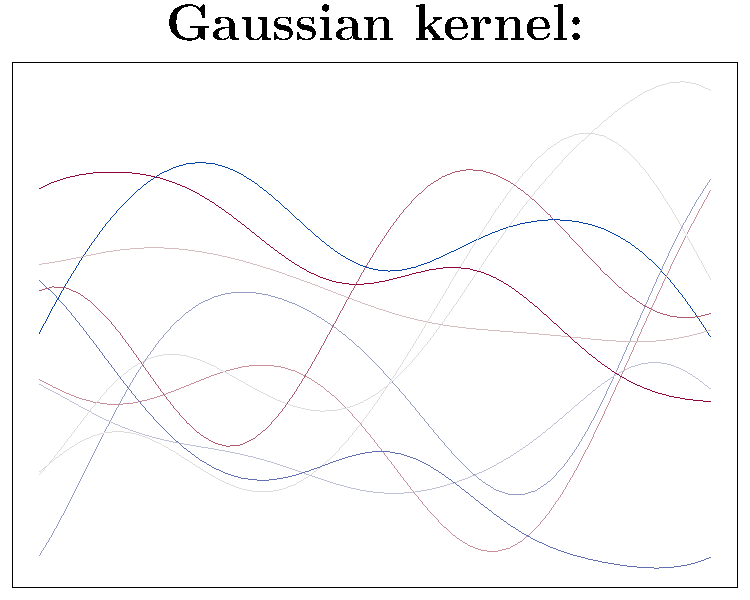
\includegraphics[height=3.8cm]{figures/R/Fig2-sim-rbf} \qquad 
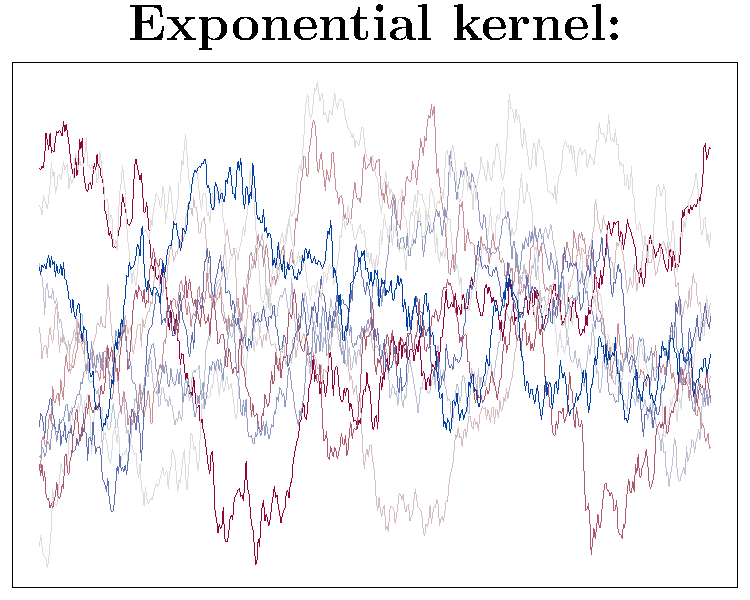
\includegraphics[height=3.8cm]{figures/R/Fig2-sim-exp}
\end{center}
\end{frame}

%%%%%%%%%%%%%%%%%%%%%%%%%%%%%%%%%%%%%%%%%%%%%%%%%%%%%%
\begin{frame}{}
It thus has \alert{a huge impact on the model}:\\ 
\begin{center}
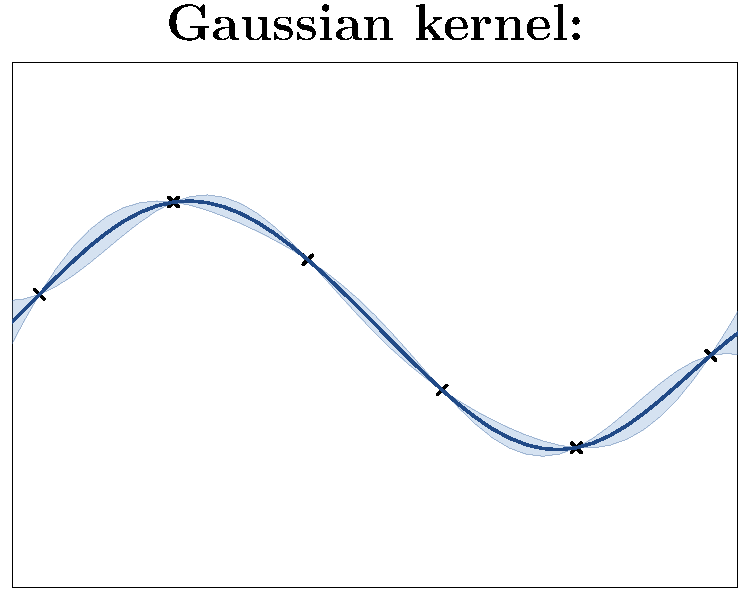
\includegraphics[height=3.9cm]{figures/R/Fig2-GP-rbf} \qquad 
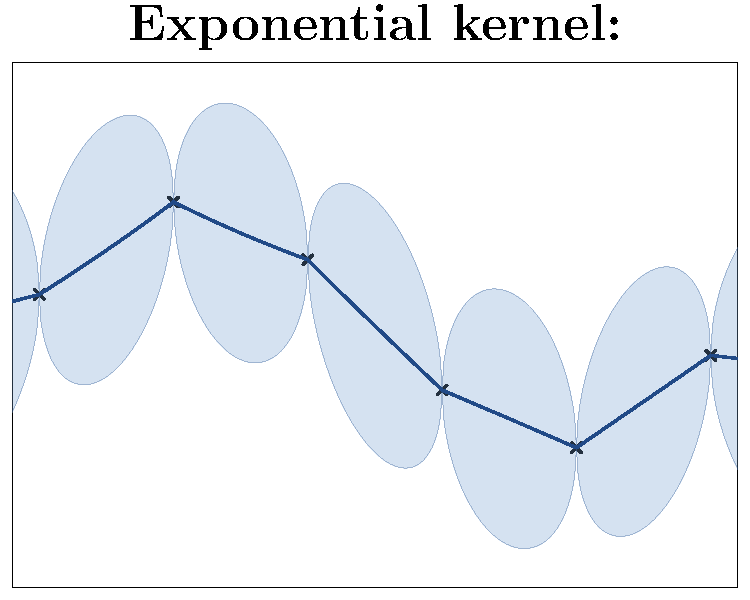
\includegraphics[height=3.9cm]{figures/R/Fig2-GP-exp}
\end{center}
\end{frame}

%%%%%%%%%%%%%%%%%%%%%%%%%%%%%%%%%%%%%%%%%%%%%%%%%%%%%%
\begin{frame}{}
There is no model/kernel that is intrinsically better... it depends on the data! \\
\vspace{5mm}
The kernel has to be chosen accordingly to our prior belief on the behaviour of the function to study:
\begin{itemize}
  \item is it continuous, differentiable, how many times?
  \item is it stationary ?
  \item ...
\end{itemize}
\vspace{5mm}
Furthermore, it is possible to introduce rescaling parameters to adjust the prior distribution to our belief.
\end{frame}

%%%%%%%%%%%%%%%%%%%%%%%%%%%%%%%%%%%%%%%%%%%%%%%%%%%%%%
\begin{frame}{}
For $d \geq 2$, there can be one rescaling parameter per dimension:
\begin{equation*}
  \Ni{x-y}{\theta} = \left( \sum_{i=1}^d \frac{(x_i-y_i)^2}{\theta_i^2} \right)^{1/2}.
\end{equation*}
\vspace{2mm}
\scriptsize
\begin{tabular}{rlN}
        squared exp. & $\displaystyle k(x,y) = \sigma^2 \exp \left(- \frac12 \Ni{x-y}{\theta}^2 \right)$ &\\[6mm]
        Matern 5/2 & $\displaystyle k(x,y) = \sigma^2 \left(1 + \sqrt{5}\Ni{x-y}{\theta} + \frac{5}{3}\Ni{x-y}{\theta}^2 \right) \exp \left(- \sqrt{5}\Ni{x-y}{\theta} \right)$ &\\[6mm]
        Matern 3/2 & $\displaystyle k(x,y) = \sigma^2 \left(1 + \sqrt{3}\Ni{x-y}{\theta} \right) \exp \left(- \sqrt{3}\Ni{x-y}{\theta}  \right)$ &\\[6mm]
        exponential & $\displaystyle k(x,y) = \sigma^2 \exp \left(- \Ni{x-y}{\theta} \right)$ 
\end{tabular}
\normalsize
\\ \vspace{5mm} \
If all $\theta_i$ are equal, we say that the kernel/process is \textbf{isotropic}.
\end{frame}


%%%%%%%%%%%%%%%%%%%%%%%%%%%%%%%%%%%%%%%%%%%%%%%%%%%%%%
%%%%%%%%%%%%%%%%%%%%%%%%%%%%%%%%%%%%%%%%%%%%%%%%%%%%%%
\section[Param Estim]{Parameter estimation}
%\subsection{}

%%%%%%%%%%%%%%%%%%%%%%%%%%%%%%%%%%%%%%%%%%%%%%%%%%%%%%
\begin{frame}{}
We have seen previously that the choice of the kernel and its parameters have a great influence on the model. \\ \vspace{5mm}
In order to choose a prior that is suited to the data at hand, we can consider:
\begin{itemize}
  \item minimising the model error
  \item Using maximum likelihood estimation 
\end{itemize}
We will now detail the second one.
\end{frame}

%%%%%%%%%%%%%%%%%%%%%%%%%%%%%%%%%%%%%%%%%%%%%%%%%%%%%%
\begin{frame}{}
The likelihood quantifies the adequacy between a distribution and some observations. 
\begin{definition}
Let $f_Y$ be a pdf depending on some parameters $p$ and let $y_1,\dots,y_n$ be independent observations. The \textbf{likelihood} is defined as 
\begin{equation*}
  L(p) = \prod_{i=1}^n f_Y(y_i;p).
\end{equation*} 
\end{definition}
A high value of $L(p)$ indicates the observations are likely to be drawn from $f_Y(.;p)$.
\end{frame}

%%%%%%%%%%%%%%%%%%%%%%%%%%%%%%%%%%%%%%%%%%%%%%%%%%%%%%
\begin{frame}{}
In the GPR context, we often have only \textbf{one observation} of the vector $F$. The likelihood is then:
\footnotesize
\begin{equation*}
  L(\sigma^2,\theta)= f_{Z(X)}(F;\sigma^2,\theta) = \frac{1}{\displaystyle | 2 \pi k(X,X)|^{1/2}} \exp \left(-\frac12 F^t k(X,X)^{-1} F  \right).
\end{equation*} 
\normalsize
It is thus possible to maximise $L$  with respect to the kernel's parameters in order to find a well suited prior.\\
\vspace{5mm}
In practice, %it is common to work with the concentrated log-likelihood:
% \begin{equation*}
%   \ell (\sigma^2, \theta) =  \log(|k(X,X)|) + F^t k(X,X)^{-1} F
% \end{equation*} 
% T
the value of $\sigma^2$ can be obtained analytically. Others, such as $\theta$, need numerical optimization.
\end{frame}

%%%%%%%%%%%%%%%%%%%%%%%%%%%%%%%%%%%%%%%%%%%%%%%%%%%%%%
\begin{frame}{}
\begin{example}
  We consider 100 sample from a  Mat\'ern 5/2 process with parameters $\sigma^2=1$ and $\theta = 0.2$, and $n$ observation points. We then try to recover the kernel parameters using MLE.\\ \vspace{5mm}
  \centering
  \begin{tabular}{|c|cccc|}
    \hline
    $n$ & 5 & 10 & 15 & 20 \\ \hline
    $\sigma^2$ & 1.0 (0.7) & 1.11 (0.71) & 1.03 (0.73) & 0.88 (0.60) \\
    $\theta$ & 0.20 (0.13) & 0.21 (0.07) & 0.20 (0.04) & 0.19 (0.03) \\ \hline
  \end{tabular}
\end{example}
\vspace{5mm}
MLE can be applied regardless to the dimension of the input space.
\end{frame}


%%%%%%%%%%%%%%%%%%%%%%%%%%%%%%%%%%%%%%%%%%%%%%%%%%%%%%
%%%%%%%%%%%%%%%%%%%%%%%%%%%%%%%%%%%%%%%%%%%%%%%%%%%%%%
\section{Model validation}
%\subsection{}

%%%%%%%%%%%%%%%%%%%%%%%%%%%%%%%%%%%%%%%%%%%%%%%%%%%%%%
\begin{frame}{}
We have seen that given some observations $F=f(X)$, it is very easy to build lots of models, either by changing the kernel parameters or the kernel itself.\\ 
\vspace{5mm}
The interesting question is how to get a good model:
\begin{itemize}
  \item What is a good model?
  \item How to measure it?
\end{itemize}
\end{frame}

%%%%%%%%%%%%%%%%%%%%%%%%%%%%%%%%%%%%%%%%%%%%%%%%%%%%%%
\begin{frame}{}
The idea is to compare the model predictions with real values on new data. 
\begin{center}
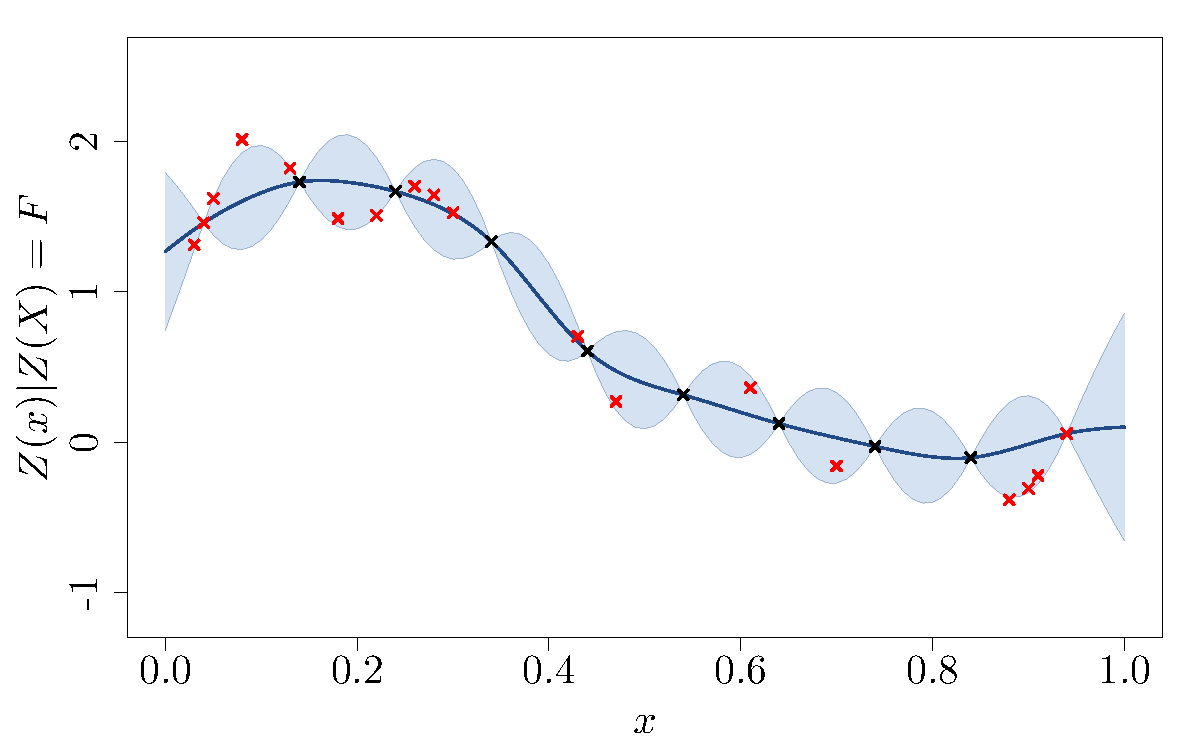
\includegraphics[height=4.5cm]{figures/R/VALID_testset}
\end{center}
\vspace{3mm}
Since GPR models provide a mean and a covariance structure for the error they both have to be assessed.
\end{frame}

%%%%%%%%%%%%%%%%%%%%%%%%%%%%%%%%%%%%%%%%%%%%%%%%%%%%%%
\begin{frame}{}
Let $X_t$ be the test set and $F_t=f(X_t)$ be the associated observations.\\ \vspace{5mm}
The accuracy of the mean can be measured by computing: 
\begin{equation*}
  \begin{split}
    \text{Mean Square Error\qquad}& MSE = \mathrm{mean} ((F_t - m(X_t))^2) \\
    \text{A ``normalised'' criterion\qquad}& Q_2 = 1 - \frac{\sum (F_t - m(X_t))^2}{\sum (F_t - \mathrm{mean}(F_t))^2} 
  \end{split}
\end{equation*}
\\ \ \\
On the above example we get $MSE = 0.038$ and $Q_2 = 0.95$.
\end{frame}

%%%%%%%%%%%%%%%%%%%%%%%%%%%%%%%%%%%%%%%%%%%%%%%%%%%%%%
\begin{frame}{}
The predicted distribution can be tested by normalising the residuals. \\ \vspace{3mm}
According to the model, $F_t \sim \mathcal{N}(m(X_t),c(X_t,X_t))$.\\ \vspace{3mm}
$c(X_t,X_t)^{-1/2}(F_t-m(X_t)) $ should thus be independents $\mathcal{N}(0,1)$:
\begin{center}
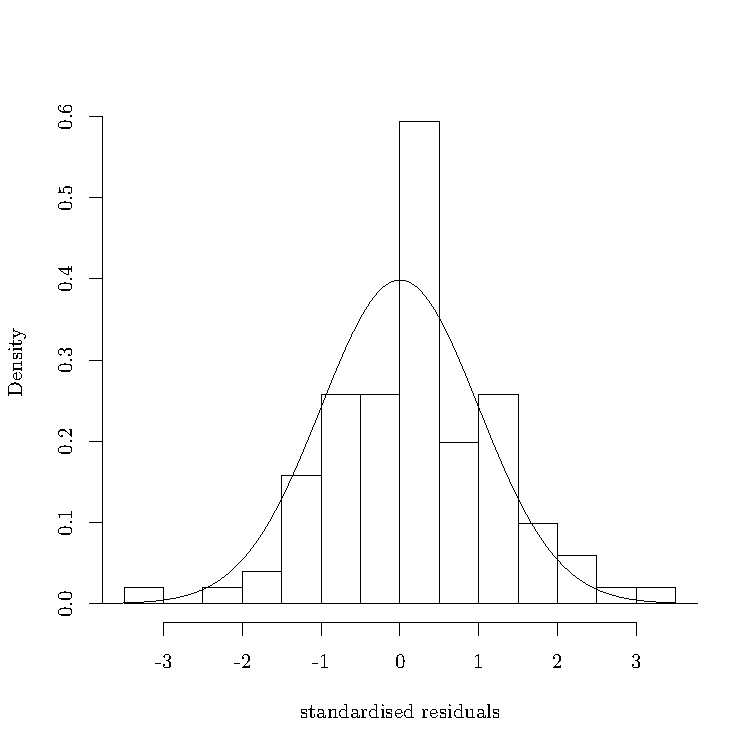
\includegraphics[height=5cm]{figures/R/VALID_hist} \qquad
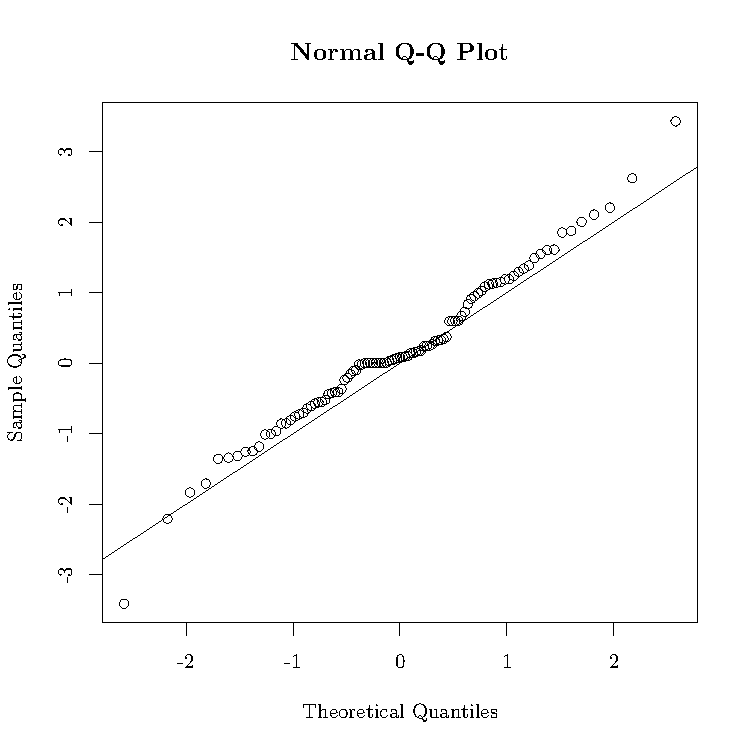
\includegraphics[height=5cm]{figures/R/VALID_qqplot}
\end{center}
\end{frame}

%%%%%%%%%%%%%%%%%%%%%%%%%%%%%%%%%%%%%%%%%%%%%%%%%%%%%%
\begin{frame}{}
When no test set is available, another option is to consider cross validation methods such as leave-one-out. \\ \vspace{5mm}
The steps are:
\begin{enumerate}
  \item[1.] build a model based on all observations except one
  \item[2.] compute the model error at this point
\end{enumerate}
This procedure can be repeated for all the design points in order to get a vector of error.
\end{frame}

%%%%%%%%%%%%%%%%%%%%%%%%%%%%%%%%%%%%%%%%%%%%%%%%%%%%%%
\begin{frame}{}
Model to be tested:\\ \vspace{3mm}
\begin{center}
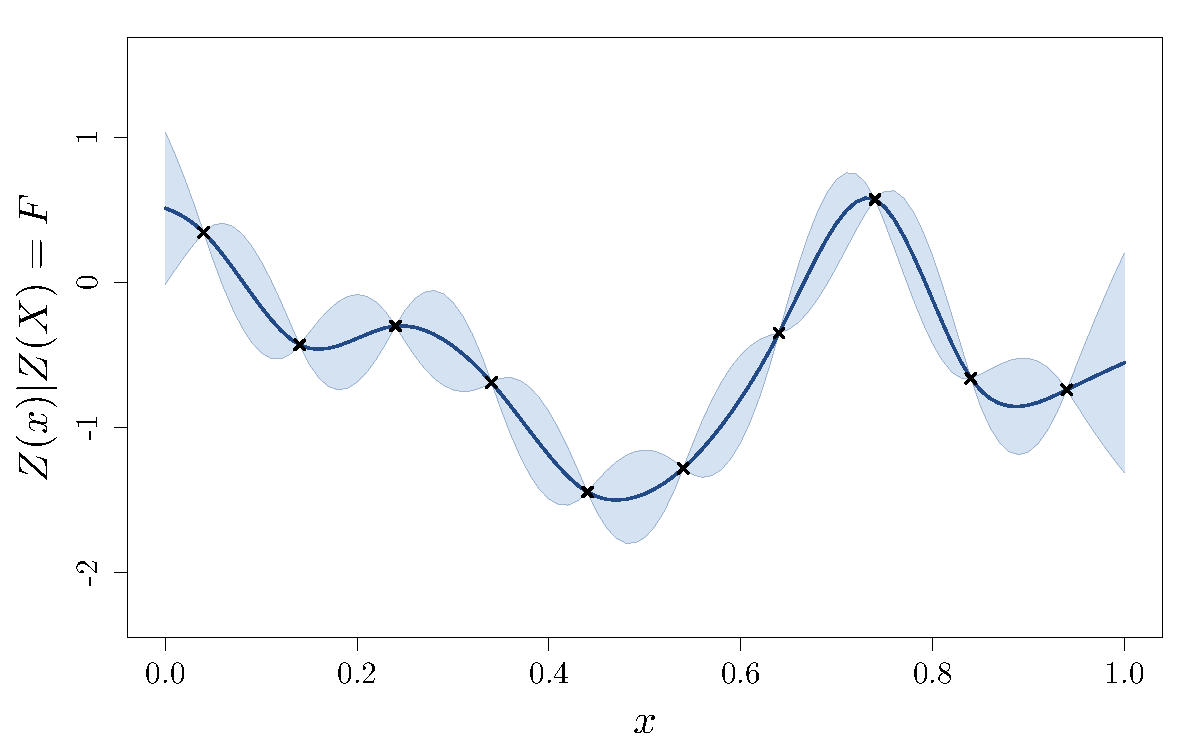
\includegraphics[height=6cm]{figures/R/VALID_crossval0}
\end{center}
\end{frame}

%%%%%%%%%%%%%%%%%%%%%%%%%%%%%%%%%%%%%%%%%%%%%%%%%%%%%%
\begin{frame}{}
Step 1:\\ \vspace{3mm}
\begin{center}
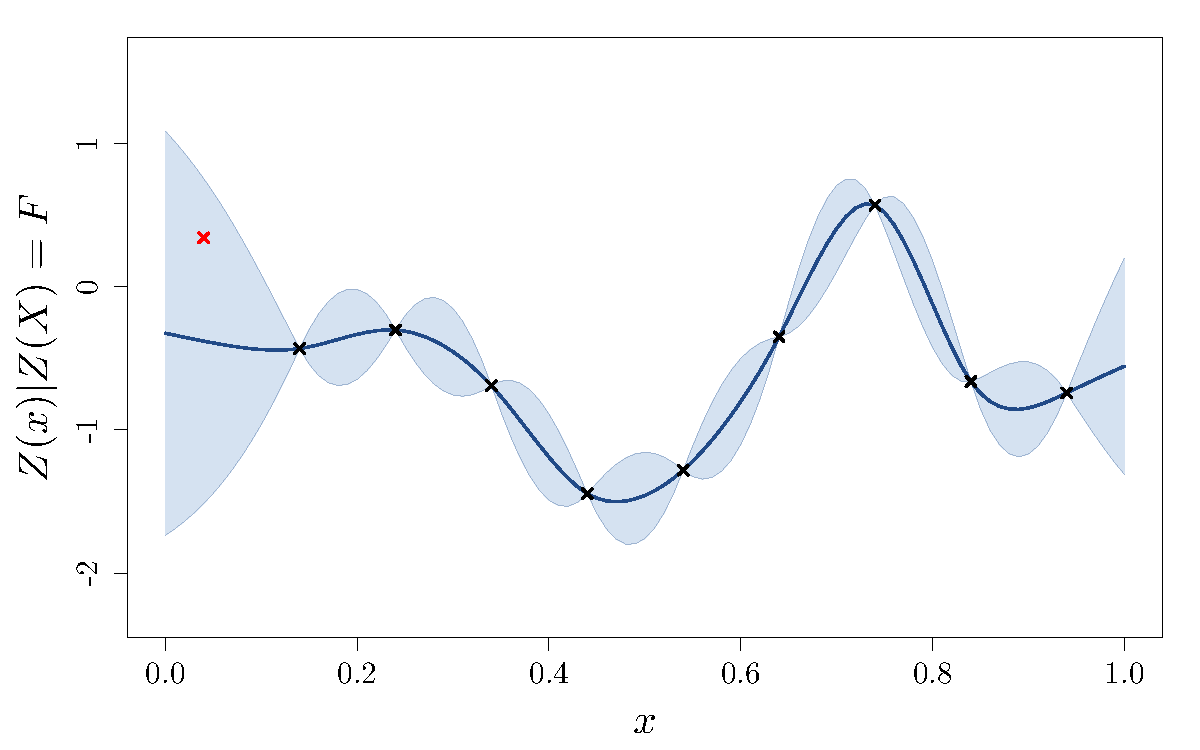
\includegraphics[height=6cm]{figures/R/VALID_crossval1}
\end{center}
\end{frame}

%%%%%%%%%%%%%%%%%%%%%%%%%%%%%%%%%%%%%%%%%%%%%%%%%%%%%%
\begin{frame}{}
Step 2:\\ \vspace{3mm}
\begin{center}
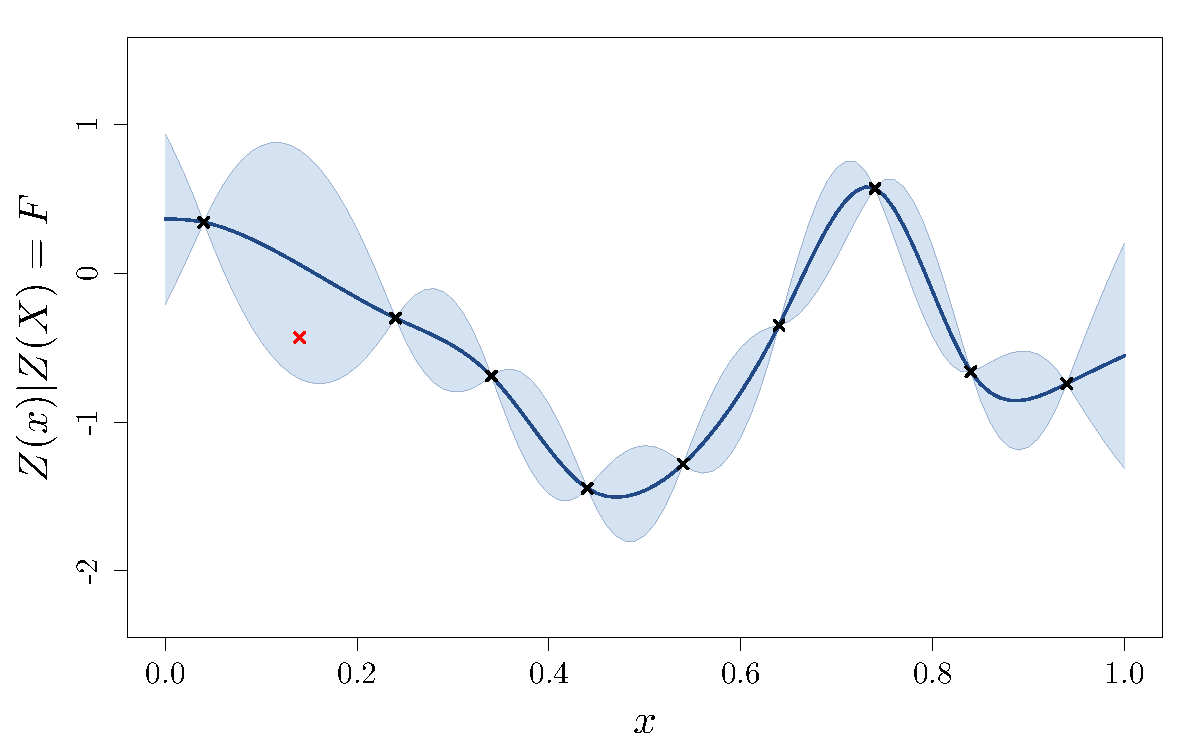
\includegraphics[height=6cm]{figures/R/VALID_crossval2}
\end{center}
\end{frame}

%%%%%%%%%%%%%%%%%%%%%%%%%%%%%%%%%%%%%%%%%%%%%%%%%%%%%%
\begin{frame}{}
Step 3:\\ \vspace{3mm}
\begin{center}
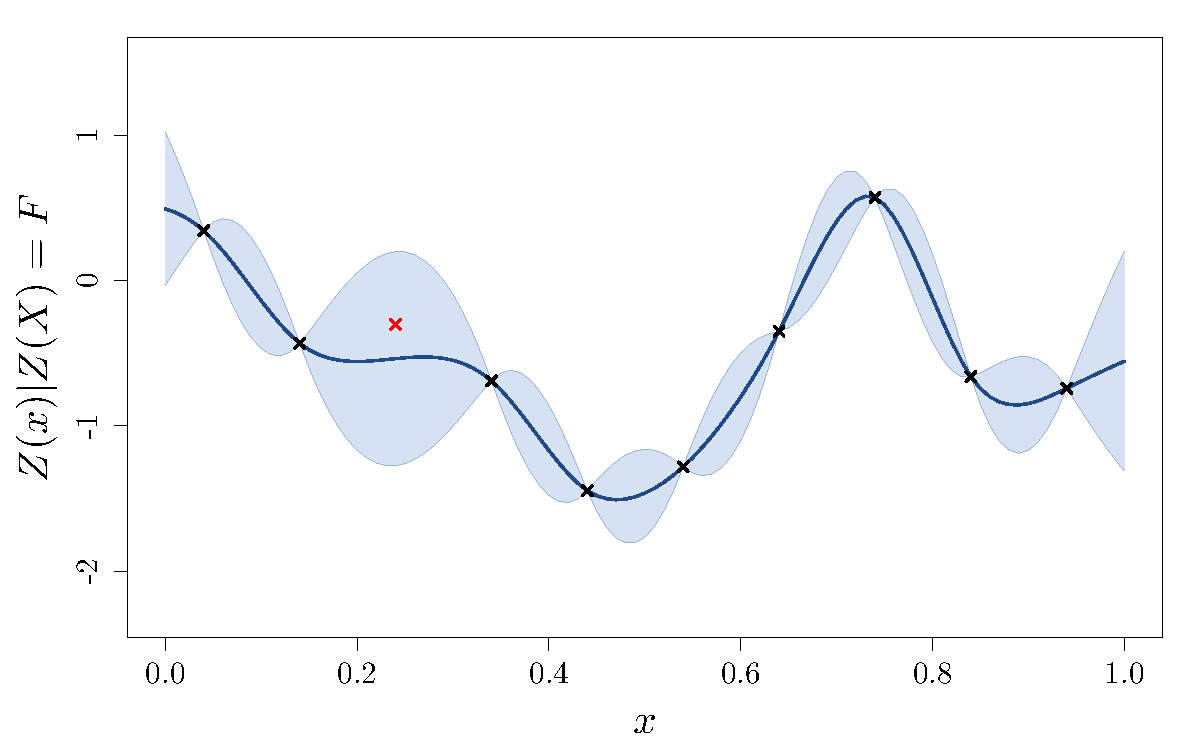
\includegraphics[height=6cm]{figures/R/VALID_crossval3}
\end{center}
\end{frame}

%%%%%%%%%%%%%%%%%%%%%%%%%%%%%%%%%%%%%%%%%%%%%%%%%%%%%%
\begin{frame}{}
On this example, we obtain $MSE = 0.24$ and $Q_2 = 0.34$. \\ \vspace{3mm} 
\begin{center}
\structure{Why doesn't the model perform as good previously?}
\end{center}

\pause
\vspace{5mm}
It turns out that the error is always computed at the `worst' location!
\end{frame}

%%%%%%%%%%%%%%%%%%%%%%%%%%%%%%%%%%%%%%%%%%%%%%%%%%%%%%
\begin{frame}{}
We can also look at the residual distribution. For leave-one-out, there is no joint distribution for the residuals so they have to be standardised independently. We obtain: 
\begin{center}
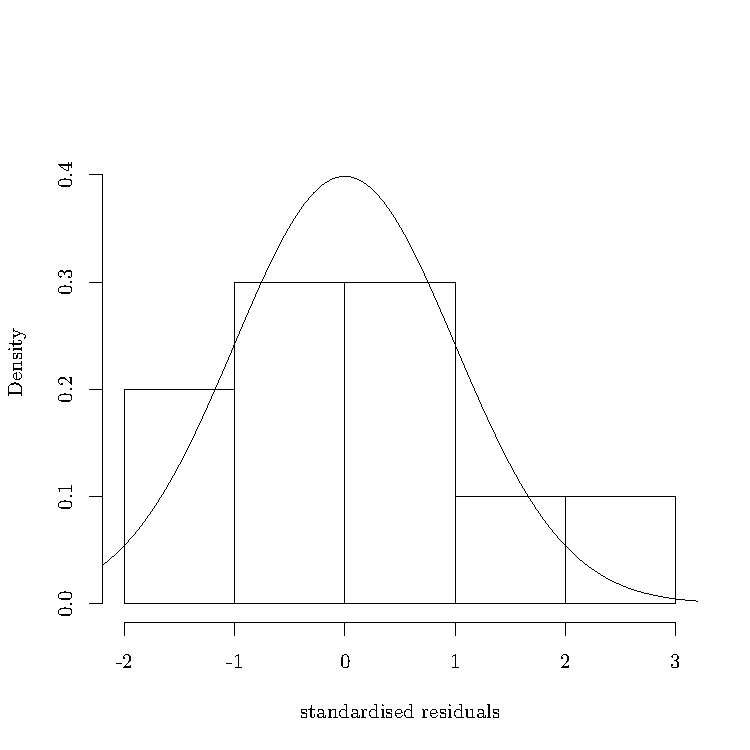
\includegraphics[height=5cm]{figures/R/VALID_crossvalhist} \qquad
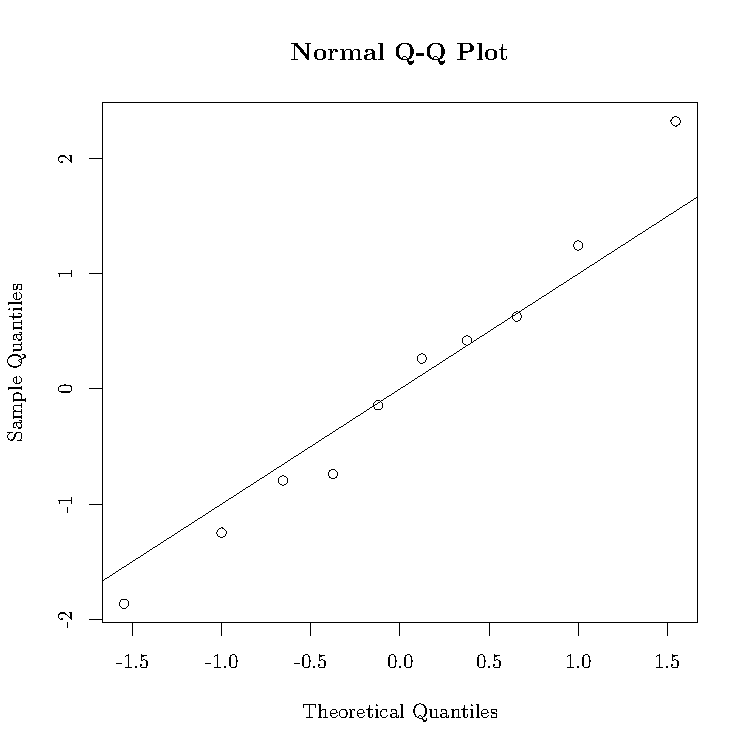
\includegraphics[height=5cm]{figures/R/VALID_crossvalqqplot}
\end{center}
\end{frame}

%%%%%%%%%%%%%%%%%%%%%%%%%%%%%%%%%%%%%%%%%%%%%%%%%%%%%%
%%%%%%%%%%%%%%%%%%%%%%%%%%%%%%%%%%%%%%%%%%%%%%%%%%%%%%
\section{Trends}
%\subsection{}

%%%%%%%%%%%%%%%%%%%%%%%%%%%%%%%%%%%%%%%%%%%%%%%%%%%%%%
\begin{frame}{}
We have seen that GPR models go back to zero if we consider a centred prior. \\ \vspace{5mm} This behaviour is not always wanted
\begin{center}
	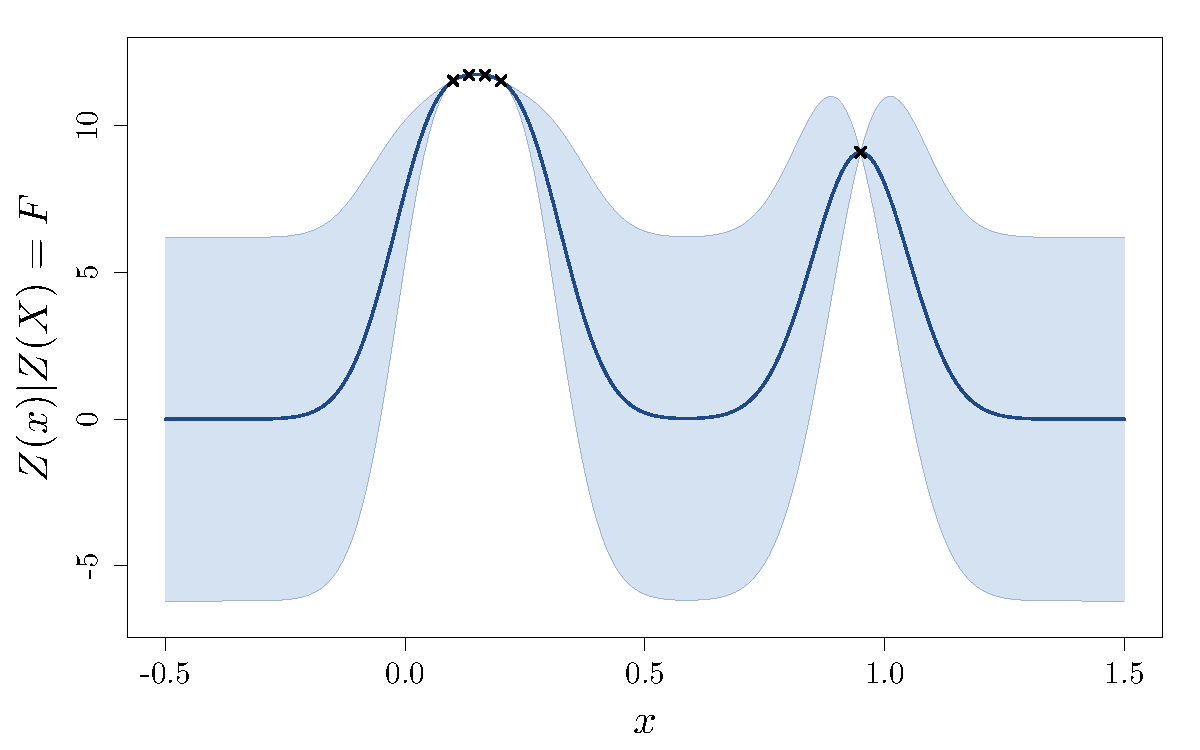
\includegraphics[height=5cm]{figures/trend_pb2}
\end{center}
\end{frame}

%%%%%%%%%%%%%%%%%%%%%%%%%%%%%%%%%%%%%%%%%%%%%%%%%%%%%%
\begin{frame}{}
We may want to introduce some trend in models... One can distinguish:
\begin{itemize}
	\item \textbf{simple kriging}: there is no trend or it is known
	\item \textbf{ordinary kriging}: the trend is a constant
	\item \textbf{universal kriging}: the trend is given by basis functions
\end{itemize}
\vspace{5mm} 
The question is how to estimate the trend coefficients. Hereafter, we will focus on ordinary kriging and write $t$ the mean value.
\end{frame}

%%%%%%%%%%%%%%%%%%%%%%%%%%%%%%%%%%%%%%%%%%%%%%%%%%%%%%
\begin{frame}{}
Basic least squares minimization gives
$$ \displaystyle \hat{t} = \frac{1}{n} \sum_{i=1}^n F_i = \frac{\mathbf{1}^t F}{\mathbf{1}^t \mathbf{1}}$$
\begin{center}
	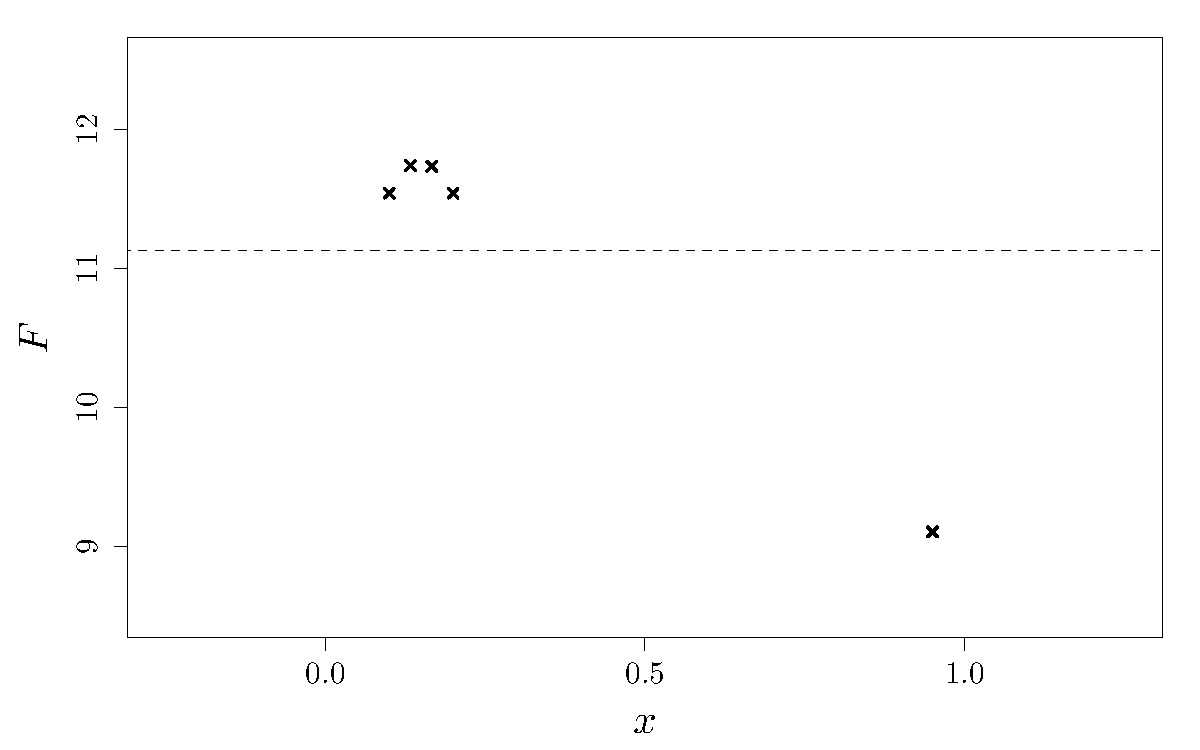
\includegraphics[height=5cm]{figures/trend_pbbasicordinary}
\end{center}
\end{frame}

%%%%%%%%%%%%%%%%%%%%%%%%%%%%%%%%%%%%%%%%%%%%%%%%%%%%%%
\begin{frame}{}
Generalised least squares is more appropriate
$$ \displaystyle \hat{t} = \frac{\mathbf{1}^t k(X,X)^{-1} F}{\mathbf{1}^t k(X,X)^{-1} \mathbf{1}}$$
\begin{center}
	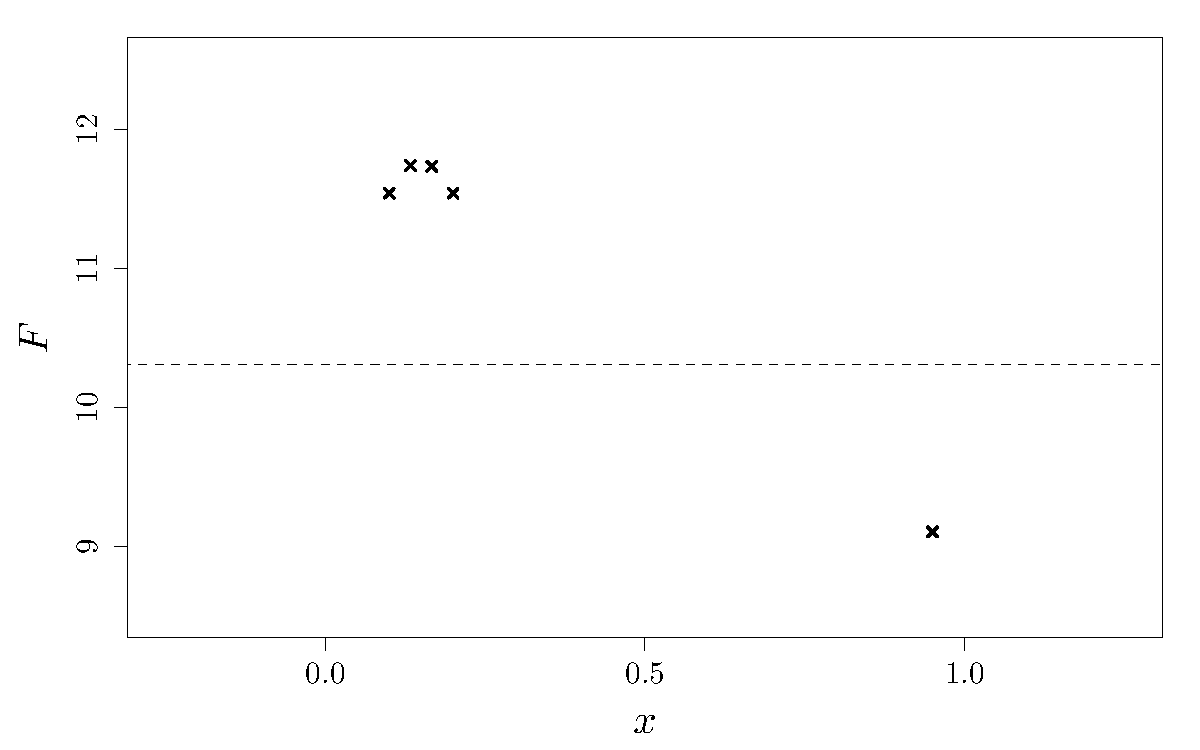
\includegraphics[height=5cm]{figures/trend_estimordinary}
\end{center}
This can be seen as maximum likelihood estimation.
\end{frame}


%%%%%%%%%%%%%%%%%%%%%%%%%%%%%%%%%%%%%%%%%%%%%%%%%%%%%%
\begin{frame}{}
The expression of the \textbf{best predictor} is given by the usual conditioning of a GP:
\begin{equation*}
m(x) = \E[Z(x)|Z(X)=F] = \hat{t} - k(x,X) k(X,X)^{-1} (F - \hat{t}) \vspace{5mm}
\end{equation*} 

Regarding the \textbf{model variance}, it must account for the estimator's variance. 
% We will use the law of total Variance :
% \begin{equation*}
% \Var[X] = \E[\Var(X|Y)] + \Var[\E(X|Y)]
% \end{equation*} 
% If we apply this to the GPR variance prediction we get:
{\small
\begin{equation*}
\begin{split}
\Var[Z(x)|Z(X)] &=  k(x,x) - k(x,X) k(X,X)^{-1} k(X,x)   \\
& \qquad + \frac{(\mathbf{1} + k(x,X)k(X,X)^{-1}\mathbf{1})^t(\mathbf{1} + k(x,X)k(X,X)^{-1}\mathbf{1})}{\mathbf{1}^t k(X,X)^{-1} \mathbf{1}} \\
\end{split}
\end{equation*} 
}
\end{frame}

%%%%%%%%%%%%%%%%%%%%%%%%%%%%%%%%%%%%%%%%%%%%%%%%%%%%%%
\begin{frame}{}
On the previous example we obtain:
\begin{center}
	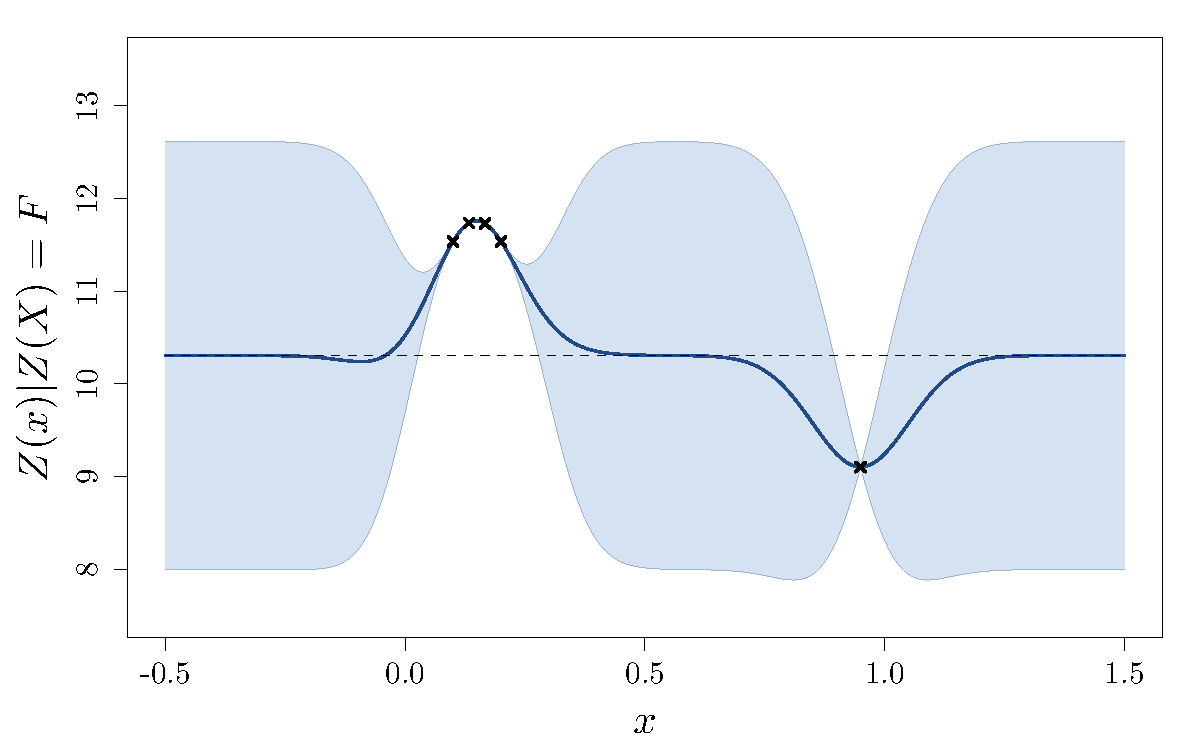
\includegraphics[height=6cm]{figures/trend_ko}
\end{center}
\end{frame}

%%%%%%%%%%%%%%%%%%%%%%%%%%%%%%%%%%%%%%%%%%%%%%%%%%%%%%
\begin{frame}{}
\begin{exampleblock}{Lab session (20 min)}
	\begin{enumerate}
		\item reload the kriging model you obtained this morning on the catapult data. (you can also use the provided one if you wish).
    \item Apply the \texttt{print()} function to your model, can you understand the output?
		\item Apply the \texttt{plot()} function to your model to get some cross validation diagnostics.
		\item Try changing the trend and kernel to improve the model.
		\item What location can you suggest for the optimum?
		$$ x_1 = \qquad,\ x_2 = \qquad,\ x_3 = \qquad,\ x_4 = \qquad.$$
    Run the simulator at that location, is there an improvement?
	\end{enumerate}
\end{exampleblock}
\end{frame}

% %%%%%%%%%%%%%%%%%%%%%%%%%%%%%%%%%%%%%%%%%%%%%%%%%%%%%%
% \begin{frame}{}
% and for a Brownian kernel:
% \begin{center}
% 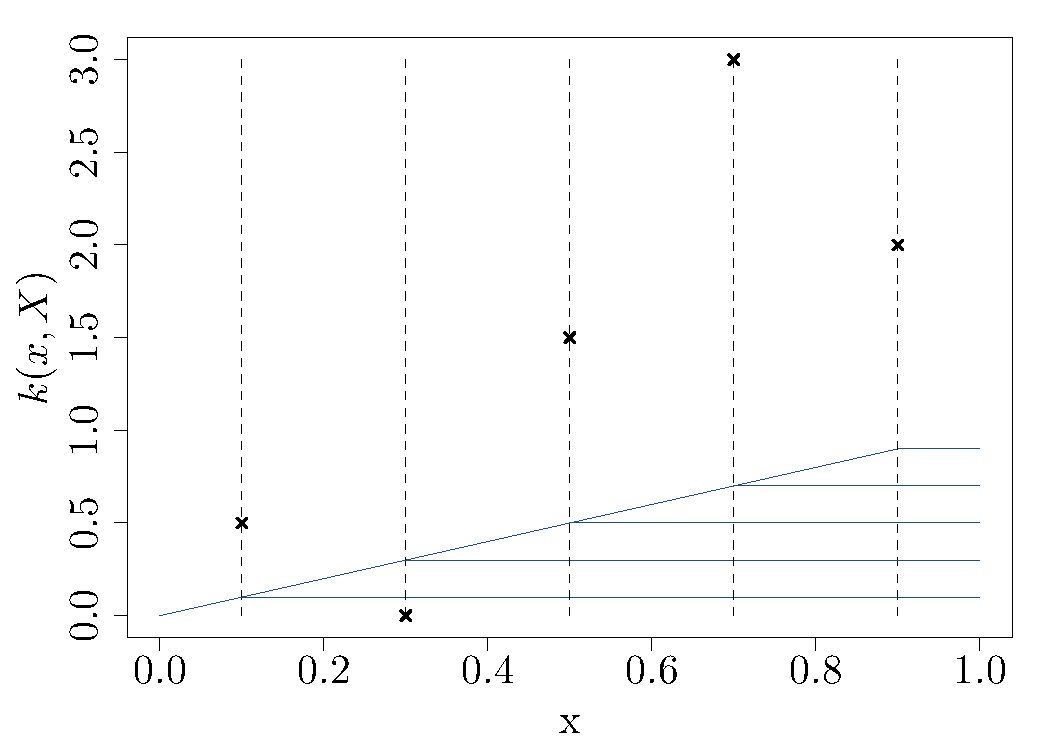
\includegraphics[height=4cm]{figures/R/ch34_basisfuncBrown}
% 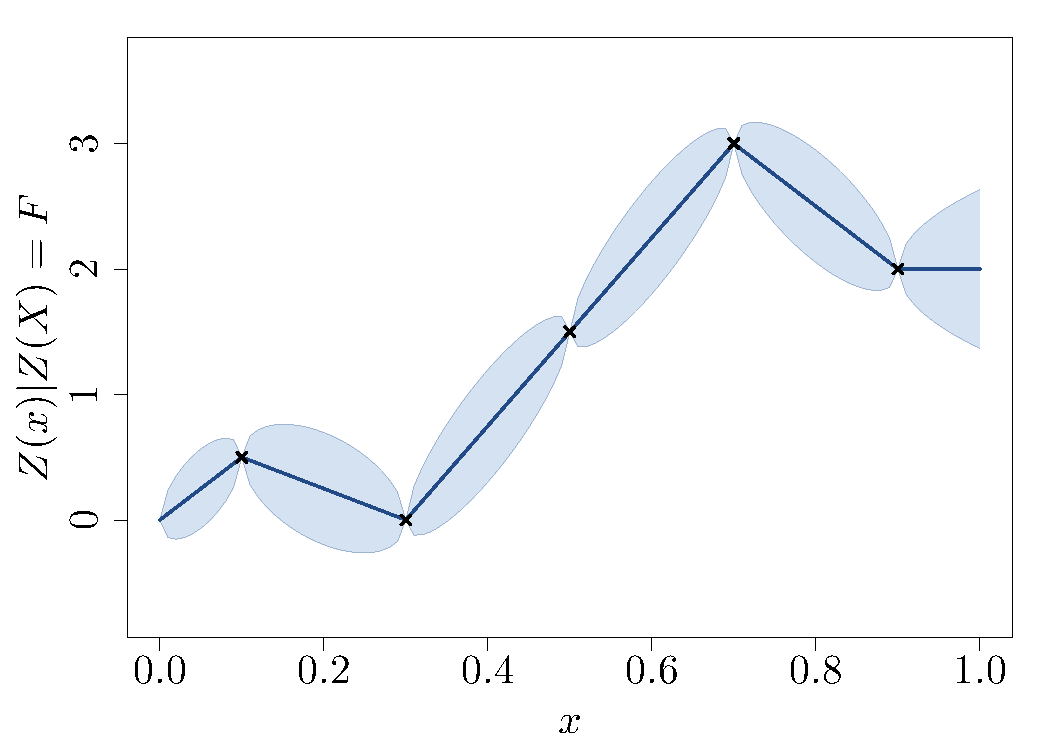
\includegraphics[height=4cm]{figures/R/ch34_GPRbasisfuncBrown}
% \end{center}
% \end{frame}


%%%%%%%%%%%%%%%%%%%%%%%%%%%%%%%%%%%%%%%%%%%%%%%%%%%%%%
%%%%%%%%%%%%%%%%%%%%%%%%%%%%%%%%%%%%%%%%%%%%%%%%%%%%%%
\section[Optimization]{Application to optimization}
%\subsection{}

%%%%%%%%%%%%%%%%%%%%%%%%%%%%%%%%%%%%%%%%%%%%%%%%%%%%%%
\begin{frame}{Framework}
  \begin{figure}
    \centering \sf
    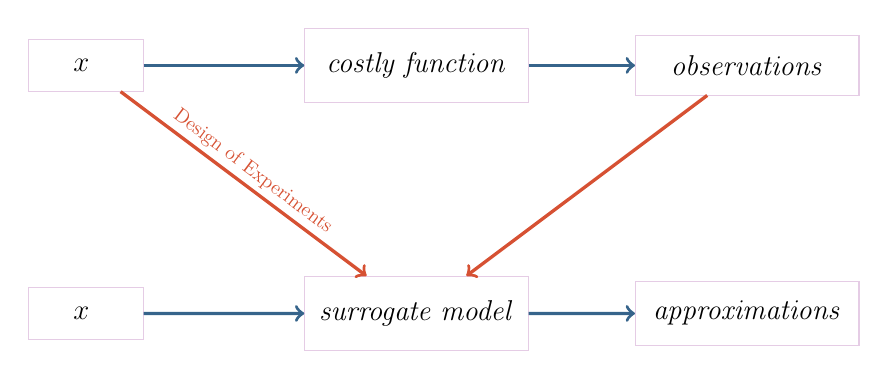
\begin{tikzpicture}[scale=0.7, every node/.style={scale=0.6}]
     
      % \tikzstyle{Sim}=[rectangle, draw=MonBleu!20, fill=MonBleu!0];
      % \tikzstyle{Meta}=[rectangle, draw=Orange!40, fill=MonBleu!0];
      \tikzstyle{Mes}=[rectangle, draw=violet!20, fill=violet!0];

        \node[Mes](MesIn) at (-6, 0) {
          \parbox{2.2cm}{ % 
            \centering
            \LARGE 
            \vspace{3mm}
            $x$
            \vspace{3mm}
          }};

        \node[Mes](Mes) at (0, 0) {
          \parbox{4.5cm}{ % 
            \centering
            \LARGE 
            \vspace{4mm}
            \textit{costly function}\\
            \vspace{4mm}
          }};
        
        \node[Mes](MesOut) at (6, 0) {
        \parbox{4.5cm}{ % 
            \centering
            \LARGE 
            \vspace{3mm}
          \textit{observations}\\
            \vspace{3mm}
        }};
        \draw[->, very thick, draw=MonBleu] (MesIn) -- (Mes.west);
        \draw[->, very thick, draw=MonBleu] (Mes) -- (MesOut.west);
        
        \node[Mes](MetaIn) at (-6, -4.5) {
          \parbox{2.2cm}{ % 
          \centering
            \LARGE 
            \vspace{3mm}
            $x$
            \vspace{3mm}
          }};
        
        \node[Mes](Meta) at (0, -4.5) {
          \parbox{4.5cm}{ % 
            \centering
            \LARGE 
            \vspace{4mm}
            \textit{surrogate model}\\
            \vspace{4mm}
          }};
        
        \node[Mes](MetaOut) at (6.0, -4.5) {
        \parbox{4.5cm}{ % 
            \centering
            \LARGE 
            \vspace{3mm}
          \textit{approximations}\\
            \vspace{3mm}
        }};
        
        \draw[->, very thick, draw=MonBleu] (MetaIn) -- (Meta.west);
        \draw[->, very thick, draw=MonBleu] (Meta) -- (MetaOut.west);
 
        \draw[->, very thick, draw=Orange!80] (MesIn) -- (Meta)
        node [above, midway, sloped, Orange!80] {\large Design of Experiments}; 
        \draw[->, very thick, draw=Orange!80] (MesOut)  -- (Meta);
        %node [above, midway, sloped, Orange!80] {\large réponses}; 

    \end{tikzpicture}
    \end{figure}  
\end{frame}

%%%%%%%%%%%%%%%%%%%%%%%%%%%%%%%%%%%%%%%%%%%%%%%%%%%%%%
\begin{frame}{Example : optimization}
\begin{block}{Case study}
We want to minimize the following function...
\begin{center}
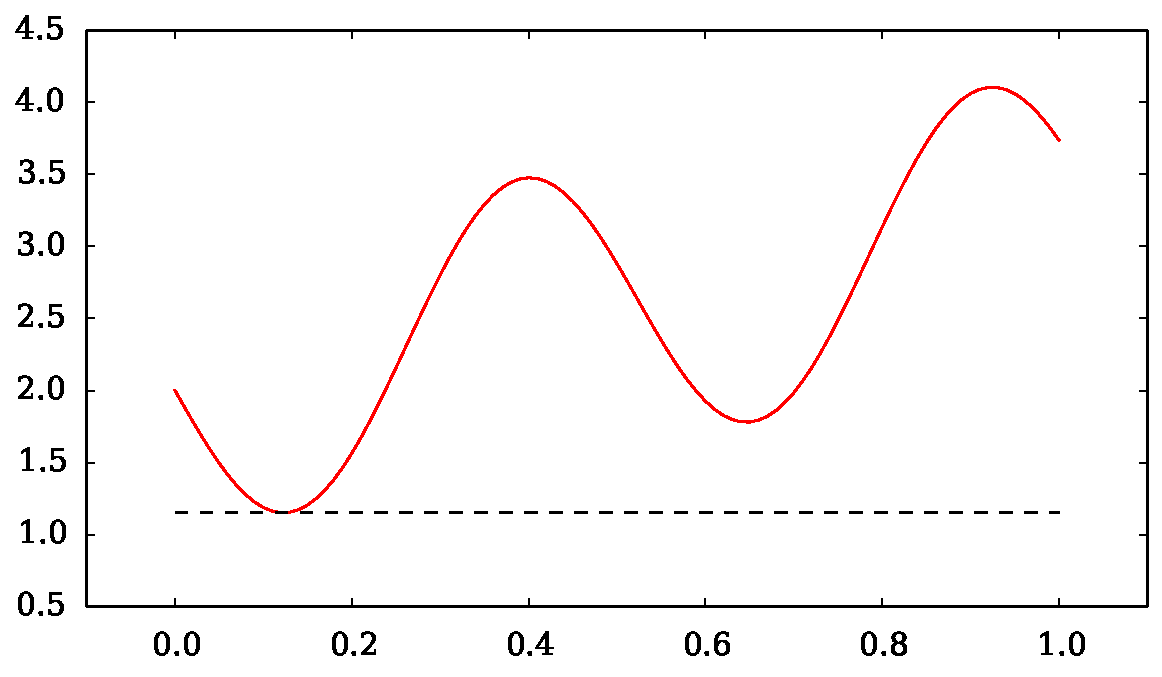
\includegraphics[height=5.5cm]{figures/python/ego_func}
\end{center}
 \end{block}
\end{frame}

%%%%%%%%%%%%%%%%%%%%%%%%%%%%%%%%%%%%%%%%%%%%%%%%%%%%%%
\begin{frame}{Example : optimization}
\begin{block}{Case study}
... which is costly.
\begin{center}
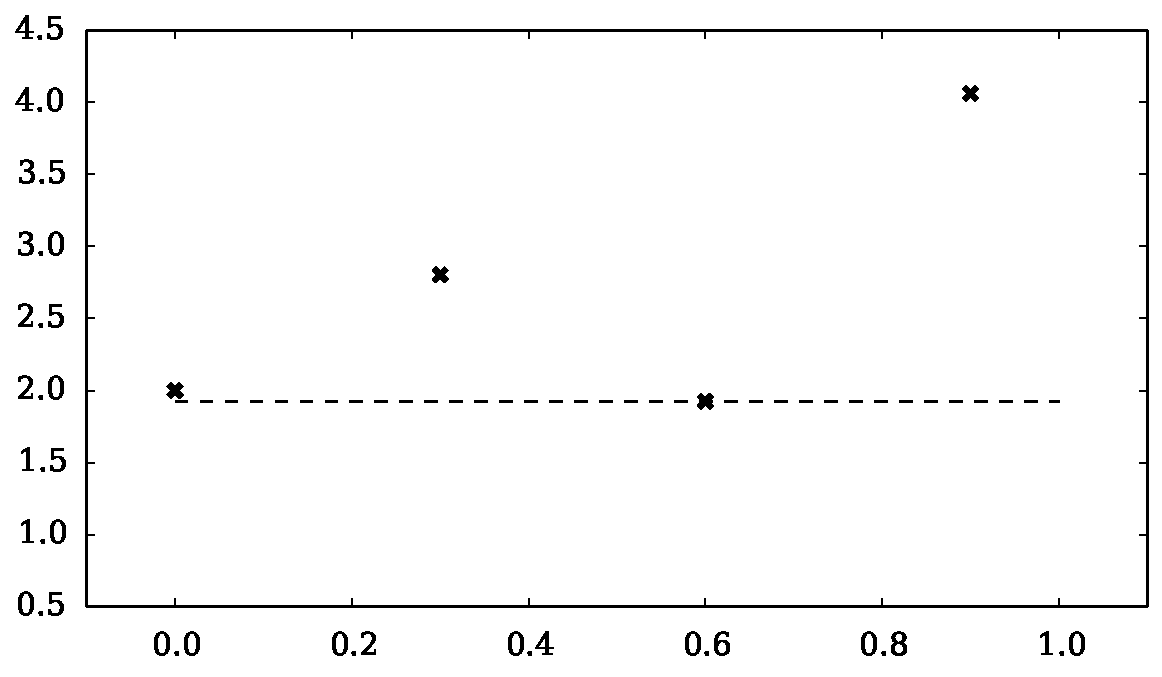
\includegraphics[height=5.5cm]{figures/python/ego_obs}
\end{center}
 \end{block}
\end{frame}

%%%%%%%%%%%%%%%%%%%%%%%%%%%%%%%%%%%%%%%%%%%%%%%%%%%%%%
\begin{frame}{Example : optimization}
We build a kriging model
\begin{center}
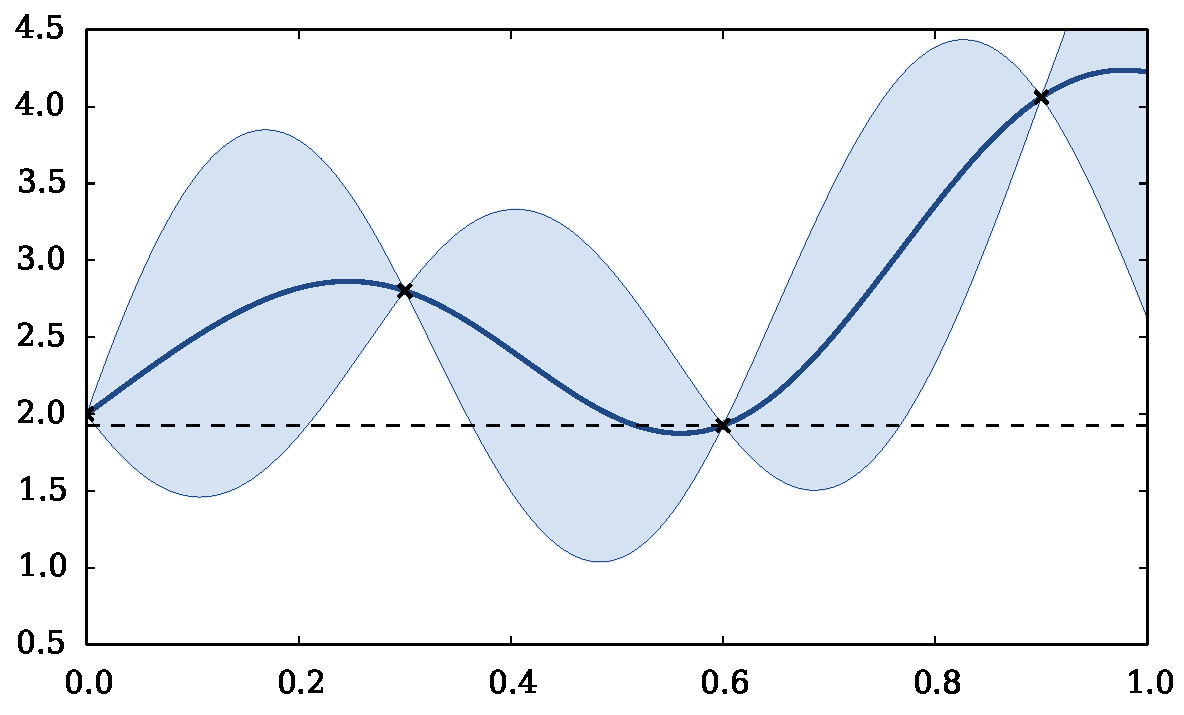
\includegraphics[height=5.5cm]{figures/python/ego_modelInit}
\end{center}
\end{frame}

%%%%%%%%%%%%%%%%%%%%%%%%%%%%%%%%%%%%%%%%%%%%%%%%%%%%%%
\begin{frame}{Example : optimization}
A common criterion is the \textbf{expected improvement}
\begin{center}
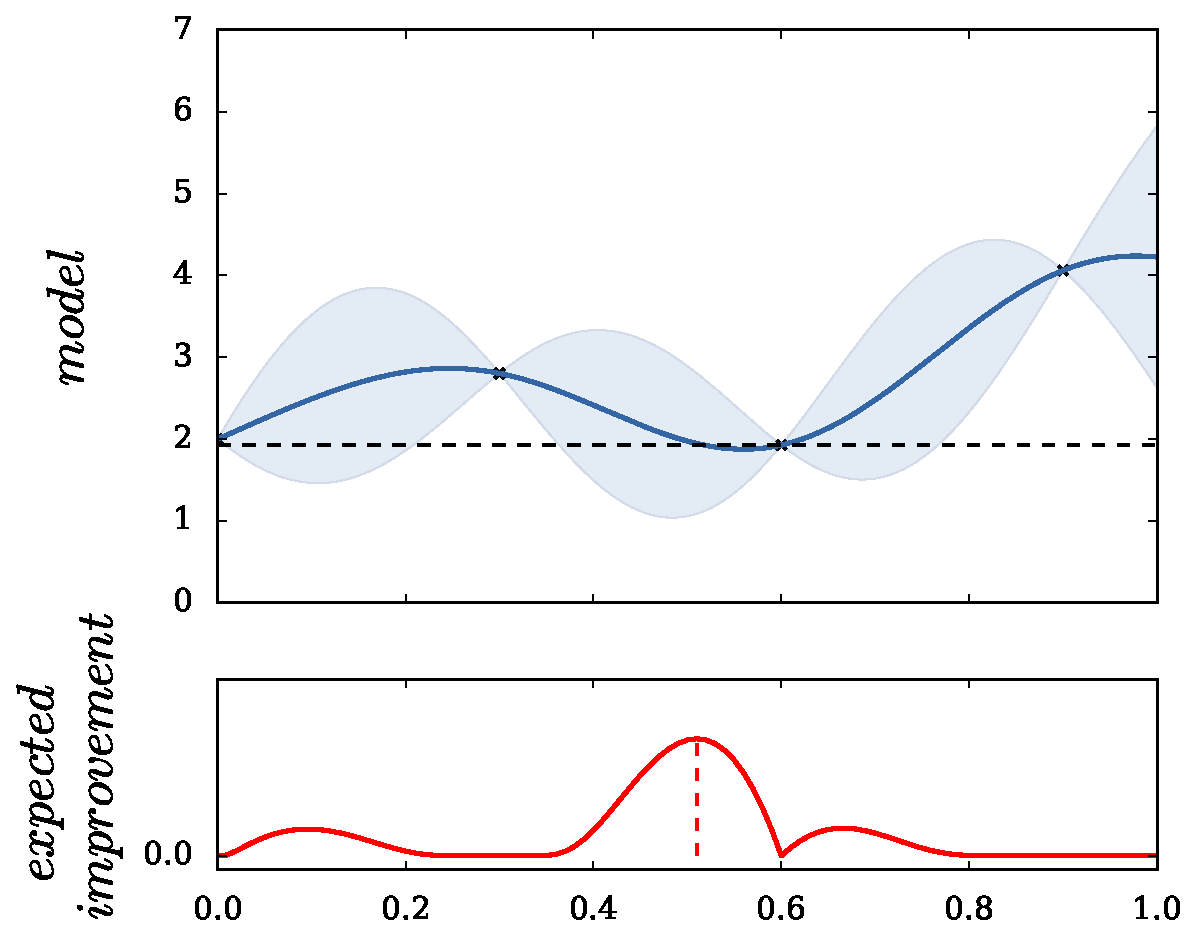
\includegraphics[height=5.5cm]{figures/python/ego_EI0}
\end{center}
$$EI(x) = \sqrt{v(x)} (u(x) cdf(u(x)) + pdf(u(x)))$$
\qquad with $ \displaystyle u(x) = \frac{\min(F) - m(x)}{\sqrt{v(x)}}$
\end{frame}

%%%%%%%%%%%%%%%%%%%%%%%%%%%%%%%%%%%%%%%%%%%%%%%%%%%%%%
\begin{frame}{Example : optimization}
We run another experiment where this criterion is maximum\\
\begin{center}
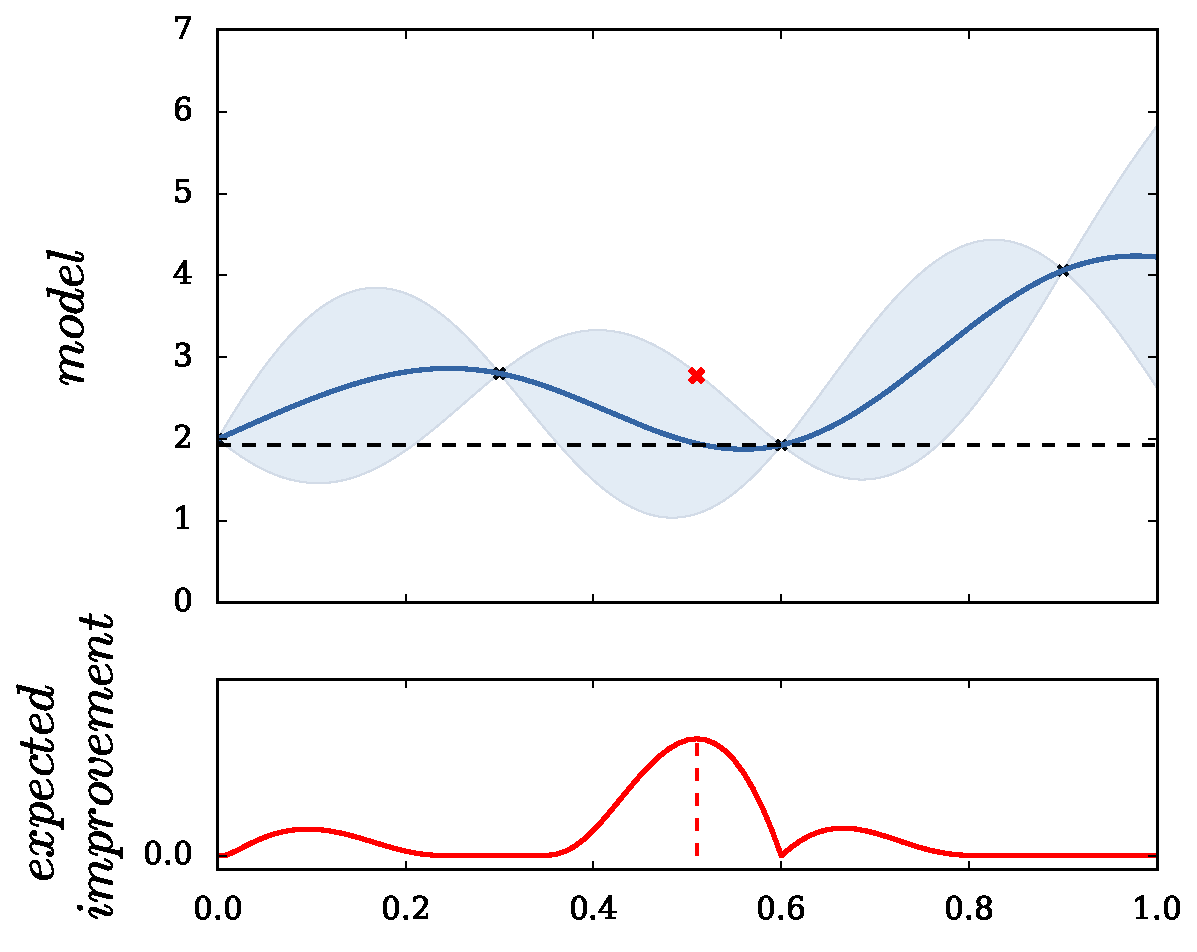
\includegraphics[height=5.5cm]{figures/python/ego_EI0bis}
\end{center}
\end{frame}

%%%%%%%%%%%%%%%%%%%%%%%%%%%%%%%%%%%%%%%%%%%%%%%%%%%%%%
\begin{frame}{Example : optimization}
\textbf{Iteration 2} :\\
\begin{center}
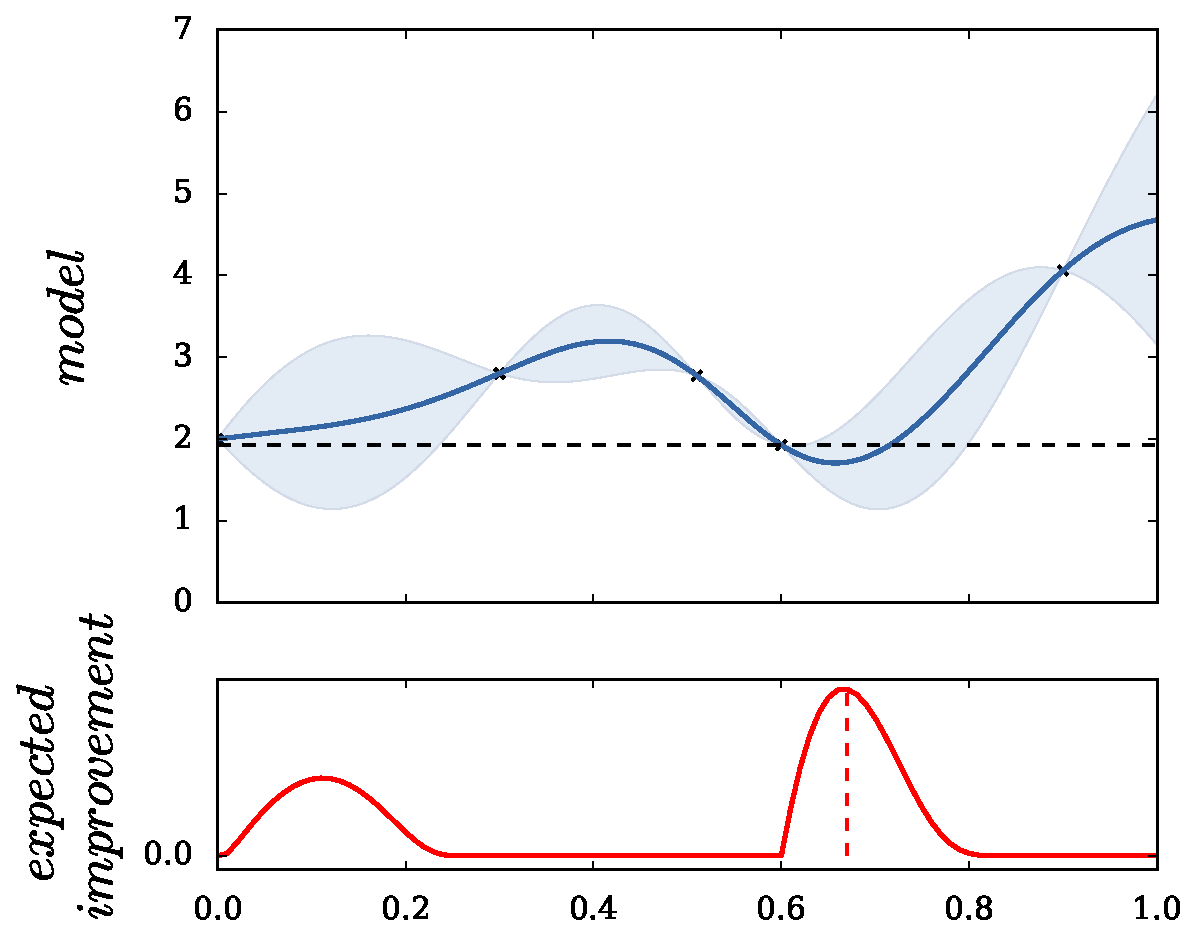
\includegraphics[height=5.5cm]{figures/python/ego_EI1}
\end{center}
\end{frame}

%%%%%%%%%%%%%%%%%%%%%%%%%%%%%%%%%%%%%%%%%%%%%%%%%%%%%%
\begin{frame}{Exemple d'application : optimisation}
\textbf{Iteration 3} :\\
\begin{center}
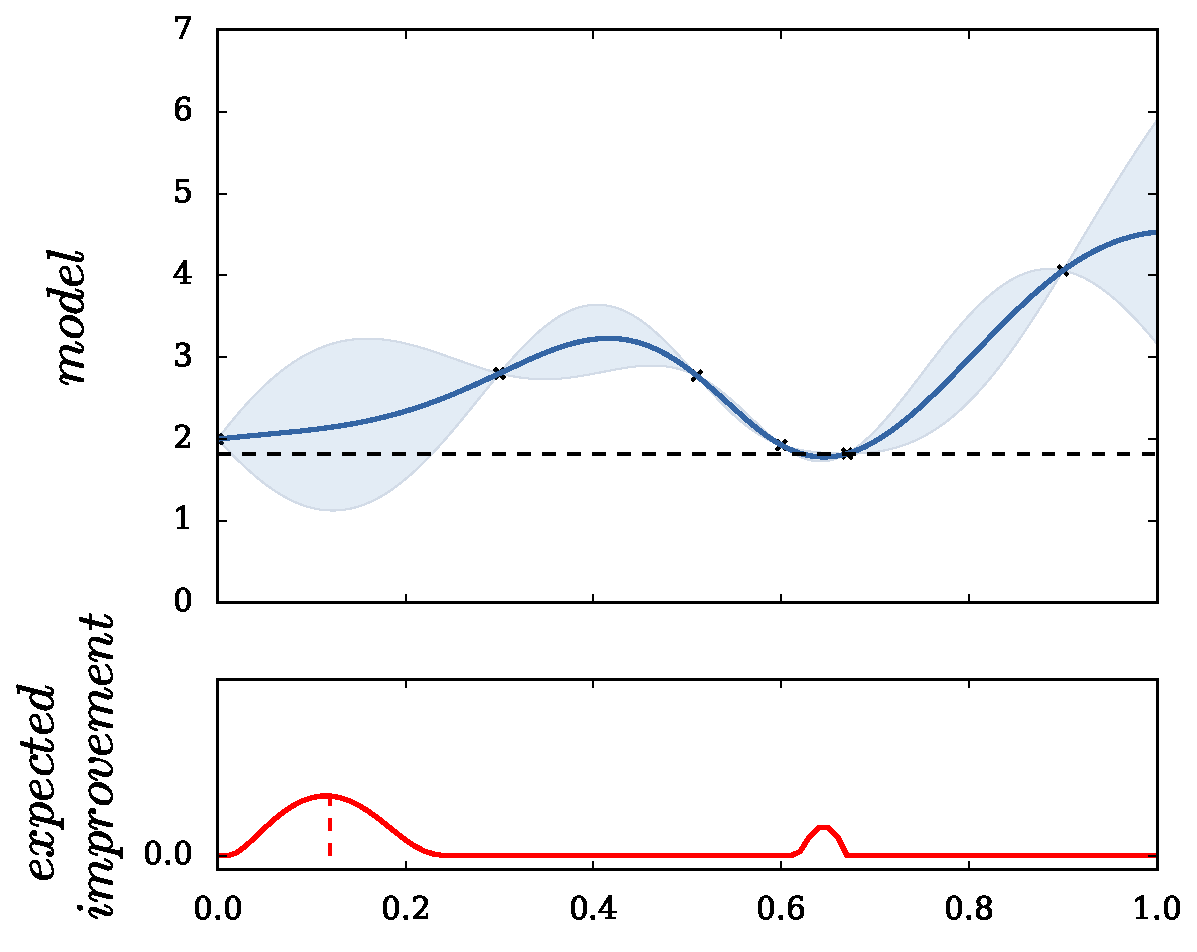
\includegraphics[height=5.5cm]{figures/python/ego_EI2}
\end{center}
\end{frame}

%%%%%%%%%%%%%%%%%%%%%%%%%%%%%%%%%%%%%%%%%%%%%%%%%%%%%%
\begin{frame}{Exemple d'application : optimisation}
\textbf{Iteration 4} :\\
\begin{center}
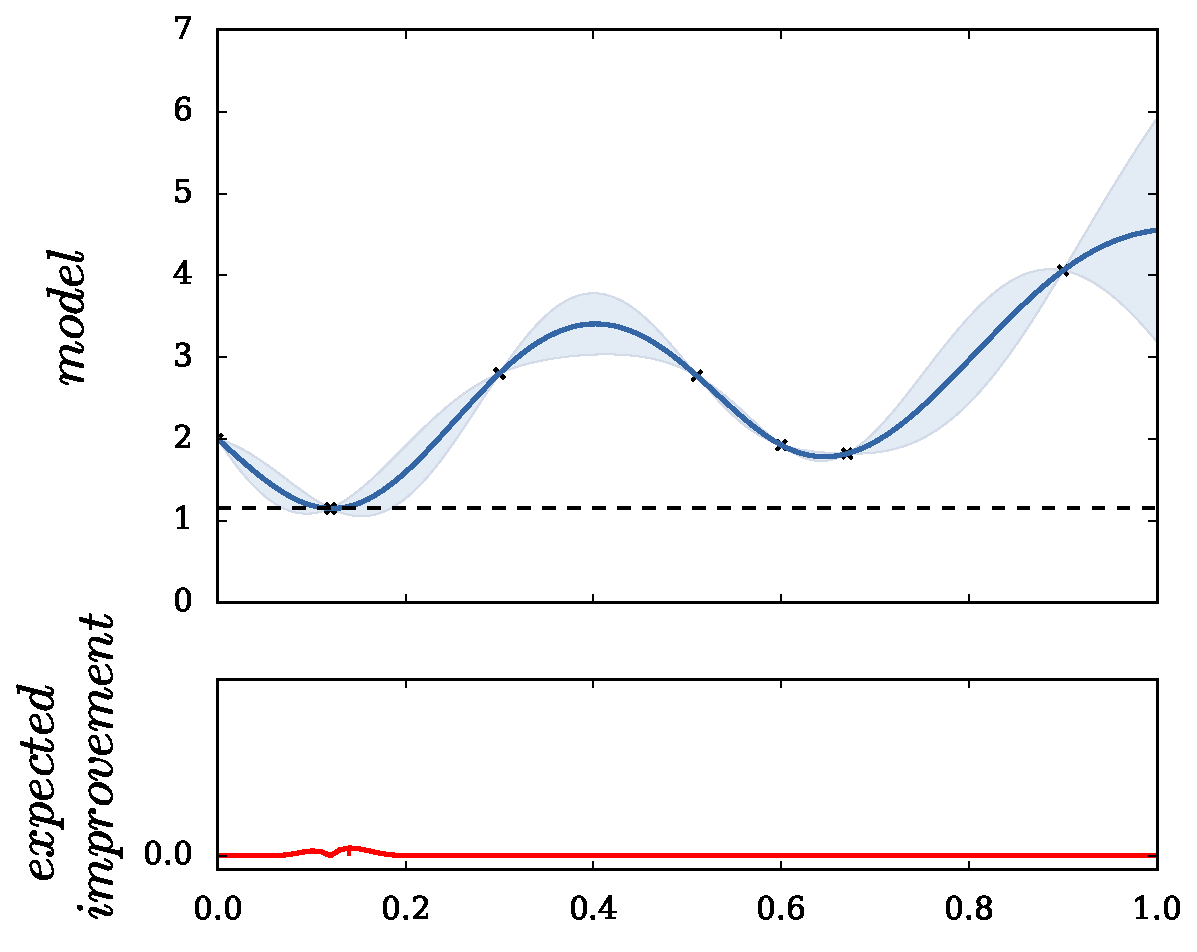
\includegraphics[height=5.5cm]{figures/python/ego_EI3}
\end{center}
\end{frame}


%%%%%%%%%%%%%%%%%%%%%%%%%%%%%%%%%%%%%%%%%%%%%%%%%%%%%%
\begin{frame}{}
\begin{exampleblock}{Lab session (20 min)}
	\begin{enumerate}
		\item We are interested here in a maximization problem... update \texttt{Y} and the kriging model to make them suitable for usual minimization algorithms. 
    \item Get the new location of the point maximising the EI (see function \texttt{max\_EI} from package \texttt{DiceOptim})
		\item Run the experiment at this location and update the model. Has the minimum been improved ?
		\item Make 20 iterations using \texttt{EGO.nsteps}. You can look at the results using the function \texttt{visualizeEGO}.
		\item What is the optimal value you obtain ?
		$$ x_1 = \qquad,\ x_2 = \qquad,\ x_3 = \qquad,\ x_4 = \qquad,\ Y_{min} = \qquad.$$
	\end{enumerate}
\end{exampleblock}
\end{frame}


%%%%%%%%%%%%%%%%%%%%%%%%%%%%%%%%%%%%%%%%%%%%%%%%%%%%%%
%%%%%%%%%%%%%%%%%%%%%%%%%%%%%%%%%%%%%%%%%%%%%%%%%%%%%%
%\section{Limitations}
%\subsection{}




%%%%%%%%%%%%%%%%%%%%%%%%%%%%%%%%%%%%%%%%%%%%%%%%%%%%%%
%%%%%%%%%%%%%%%%%%%%%%%%%%%%%%%%%%%%%%%%%%%%%%%%%%%%%%
\section{Conclusion}
%\subsection{}

%%%%%%%%%%%%%%%%%%%%%%%%%%%%%%%%%%%%%%%%%%%%%%%%%%%%%%
\begin{frame}{}
Statistical models are useful when little data is available. they allow to
  \begin{itemize}
    \item interpolate or approximate functions
    \item Compute quantities of interests (such as mean value, optimum, ...)
    \item Get some uncertainty measure
  \end{itemize}
\end{frame}

%%%%%%%%%%%%%%%%%%%%%%%%%%%%%%%%%%%%%%%%%%%%%%%%%%%%%%
\begin{frame}{}
\structure{Small Recap} We have seen that \vspace{2mm}
\begin{block}{}
\begin{itemize}
 \item Many kernels can be used to build models.
 \begin{itemize}
  \item Given some data, there is not one GP model but an infinity...
 \end{itemize} \vspace{2mm}
 \item Kernels encode the prior belief on the function to approximate.
 \begin{itemize}
  \item They should be chosen accordingly
 \end{itemize}\vspace{2mm}
 \item Model/kernel parameters can tuned to the problem at hand \vspace{2mm}
 \item GPR models do not necessarily interpolate. \vspace{2mm}
 \item Model validation is of the utmost importance
 \begin{itemize}
    \item mean \textbf{and} predicted (co-)variance
  \end{itemize}
\end{itemize}
\end{block}
\end{frame}

%%%%%%%%%%%%%%%%%%%%%%%%%%%%%%%%%%%%%%%%%%%%%%%%%%%%%%
\begin{frame}{Limitations}
The complexity of using kriging models is in building the model
\begin{itemize}
  \item $\mathcal{O}(n^2)$ for the storage footprint
  \begin{itemize}
    \item storage of the covariance matrix $k(X,X)$
  \end{itemize}
  \item $\mathcal{O}(n^3)$ for the number of operations
    \begin{itemize}
    \item inversion of the covariance matrix $k(X,X)$
  \end{itemize}
\end{itemize}
In practice, the maximum number of observation for classical models lies in the range [1000, 10000].\\
\vspace{5mm}
Another common issue is the numerical stability of the matrix inversion
\begin{itemize}
  \item pseudo-inverse
  \item nugget (or jitter)
\end{itemize}
\end{frame}

%%%%%%%%%%%%%%%%%%%%%%%%%%%%%%%%%%%%%%%%%%%%%%%%%%%%%%
%%%%%%%%%%%%%%%%%%%%%%%%%%%%%%%%%%%%%%%%%%%%%%%%%%%%%%
\section{Appendix}
%\subsection{}

%%%%%%%%%%%%%%%%%%%%%%%%%%%%%%%%%%%%%%%%%%%%%%%%%%%%%%
\begin{frame}{Approximation}
We are not always interested in models that interpolate the data. For example, if there is some observation noise: $F = f(X) + \varepsilon$.
\begin{center}
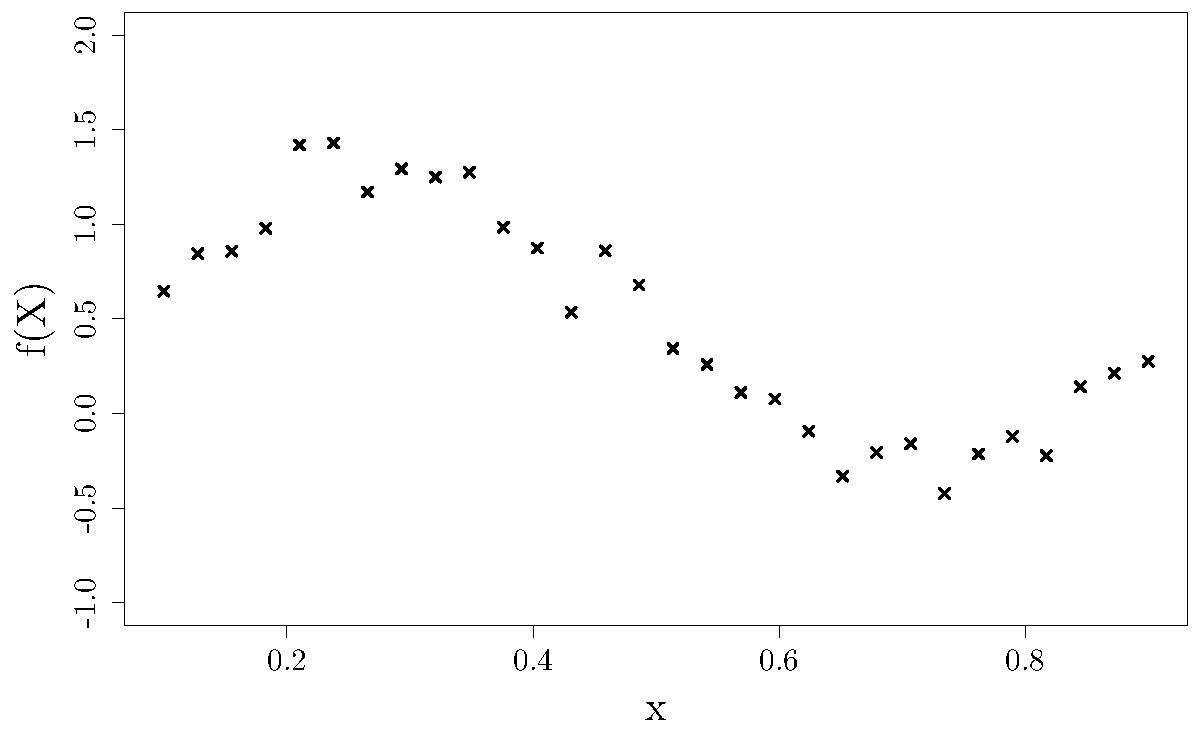
\includegraphics[height=6cm]{figures/R/noisyObs} 
\end{center}
\end{frame}

%%%%%%%%%%%%%%%%%%%%%%%%%%%%%%%%%%%%%%%%%%%%%%%%%%%%%%
\begin{frame}{Approximation}
\vspace{5mm}
Let $N$ be a process $\mathcal{N}(0,n)$ that represent the observation noise. The expressions of GPR with noise are 
\begin{equation*}
  \begin{split}
  m(x) &= \E[Z(x)|Z(X) + N(X) \shorteq F] \\
  &= k(x,X) (k(X,X)+n(X,X))^{-1} F \\ 
  & \\
  c(x,y) &= \Cov[Z(x),Z(y)|Z(X)+ N(X) \shorteq F] \\
  &= k(x,y) - k(x,X) (k(X,X)+n(X,X))^{-1} k(X,y)
\end{split}
\end{equation*}
\end{frame}

%%%%%%%%%%%%%%%%%%%%%%%%%%%%%%%%%%%%%%%%%%%%%%%%%%%%%%
\begin{frame}{Approximation}
We obtain the following model
\begin{center}
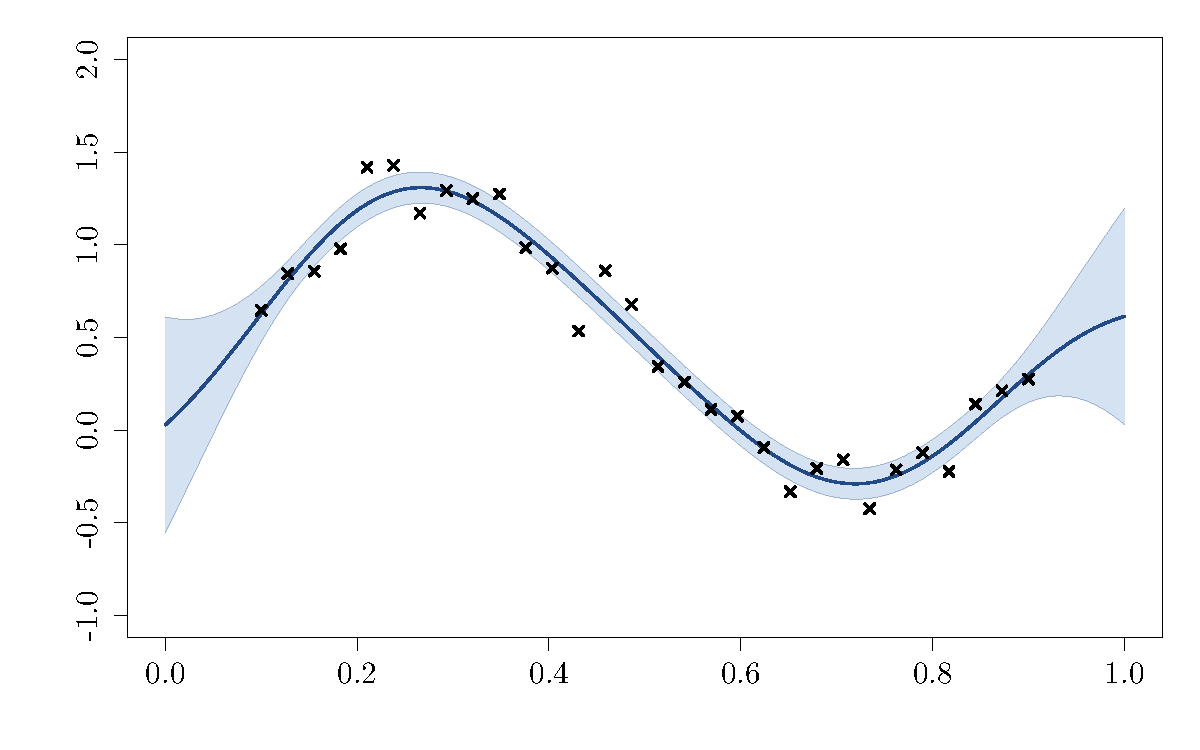
\includegraphics[height=6cm]{figures/R/noisyGPR} 
\end{center}
\end{frame}

%%%%%%%%%%%%%%%%%%%%%%%%%%%%%%%%%%%%%%%%%%%%%%%%%%%%%%
\begin{frame}{Approximation}
Influence of observation noise $\tau^2$ (for $n(x,y)=\tau^2 \delta_{x,y}$):
\begin{center}
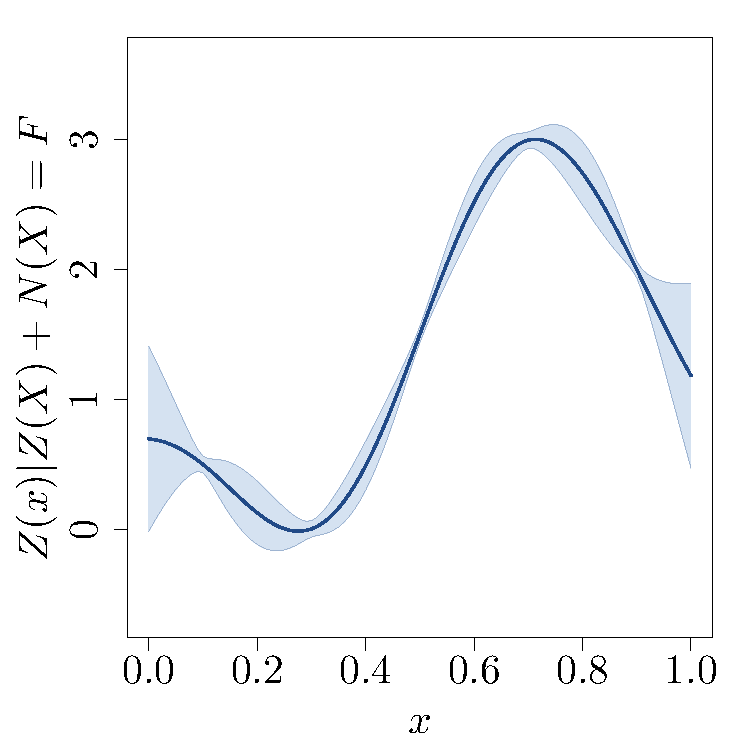
\includegraphics[height=3.5cm]{figures/R/ch34_GPRnoise0001} 
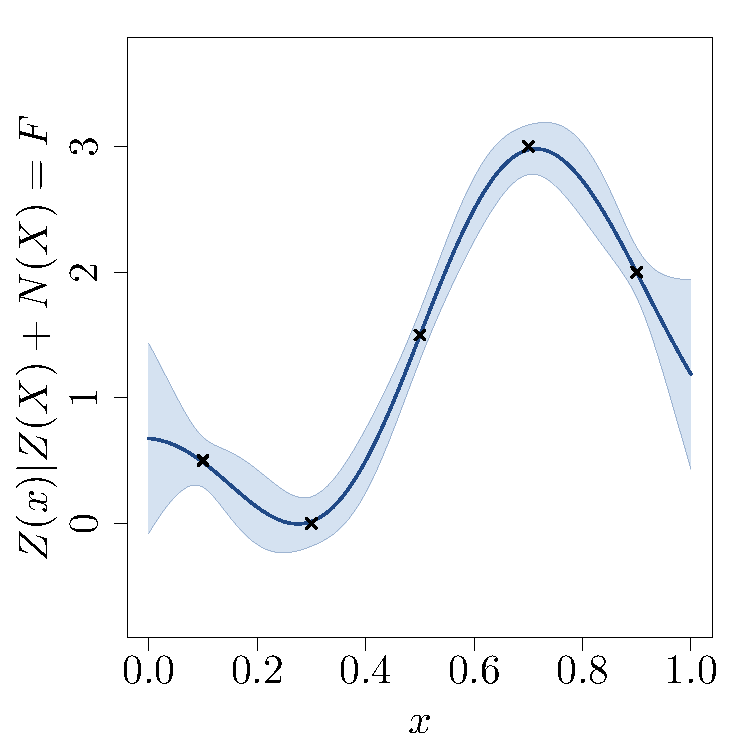
\includegraphics[height=3.5cm]{figures/R/ch34_GPRnoise001} 
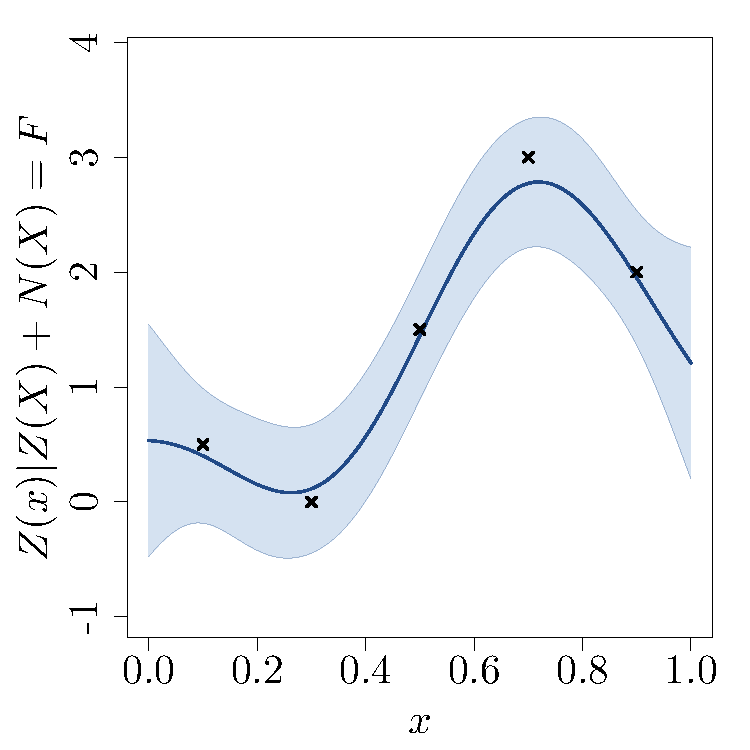
\includegraphics[height=3.5cm]{figures/R/ch34_GPRnoise01}\\
The values of $\tau^2$ are respectively 0.001, 0.01 and 0.1.
\end{center}
In practice, $\tau^2$ can be estimated with Maximum Likelihood. 
\end{frame}


%%%%%%%%%%%%%%%%%%%%%%%%%%%%%%%%%%%%%%%%%%%%%%%%%%%%%%%%%%%%%%%%%%%%%%%%%%%%%%%
%%%%%%%%%%%%%%%%%%%%%%%%%%%%%%%%%%%%%%%%%%%%%%%%%%%%%%%%%%%%%%%%%%%%%%%%%%%%%%%
%%%%%%%%%%%%%%%%%%%%%%%%%%%%%%%%%%%%%%%%%%%%%%%%%%%%%%%%%%%%%%%%%%%%%%%%%%%%%%%
%%%%%%%%%%%%%%%%%%%%%%%%%%%%%%%%%%%%%%%%%%%%%%%%%%%%%%%%%%%%%%%%%%%%%%%%%%%%%%%
\end{document}



\structure{}

\begin{center}
  \begin{tabular}{|c|cc|}

  \end{tabular}
\end{center}

###
%%%%%%%%%%%%%%%%%%%%%%%%%%%%%%%%%%%%%%%%%%%%%%%%%%%%%%
\begin{frame}{}

\end{frame}

###
\begin{block}{}

\end{block}

###
\begin{center}
\includegraphics[height=5cm]{figures/}
\end{center}

###
\begin{columns}[c]
\column{5cm}

\column{5cm}

\end{columns}
